\documentclass[letterpaper]{article}
\usepackage[margin=1in]{geometry}
\usepackage[utf8]{inputenc}
\usepackage{textcomp}
\usepackage{amssymb}
\usepackage{natbib}
\usepackage{graphicx}
\usepackage{gensymb}
\usepackage{amsthm, amsmath, mathtools}
\usepackage[dvipsnames]{xcolor}
\usepackage{enumerate}
\usepackage{mdframed}
\usepackage[most]{tcolorbox}
\usepackage{csquotes}
% https://tex.stackexchange.com/questions/13506/how-to-continue-the-framed-text-box-on-multiple-pages

\tcbuselibrary{theorems}

\newcommand{\R}{\mathbb{R}}
\newcommand{\Z}{\mathbb{Z}}
\newcommand{\N}{\mathbb{N}}
\newcommand{\Q}{\mathbb{Q}}
\newcommand{\C}{\mathbb{C}}
\newcommand{\code}[1]{\texttt{#1}}
\newcommand{\mdiamond}{$\diamondsuit$}
\newcommand{\PowerSet}{\mathcal{P}}
\newcommand{\Mod}[1]{\ (\mathrm{mod}\ #1)}
\DeclareMathOperator{\lcm}{lcm}

%\newtheorem*{theorem}{Theorem}
%\newtheorem*{definition}{Definition}
%\newtheorem*{corollary}{Corollary}
%\newtheorem*{lemma}{Lemma}
\newtheorem*{proposition}{Proposition}


\newtcbtheorem[number within=section]{theorem}{Theorem}
{colback=green!5,colframe=green!35!black,fonttitle=\bfseries}{th}

\newtcbtheorem[number within=section]{definition}{Definition}
{colback=blue!5,colframe=blue!35!black,fonttitle=\bfseries}{def}

\newtcbtheorem[number within=section]{corollary}{Corollary}
{colback=yellow!5,colframe=yellow!35!black,fonttitle=\bfseries}{cor}

\newtcbtheorem[number within=section]{lemma}{Lemma}
{colback=red!5,colframe=red!35!black,fonttitle=\bfseries}{lem}

\newtcbtheorem[number within=section]{example}{Example}
{colback=white!5,colframe=white!35!black,fonttitle=\bfseries}{def}

\newtcbtheorem[number within=section]{note}{Important Note}{
        enhanced,
        sharp corners,
        attach boxed title to top left={
            xshift=-1mm,
            yshift=-5mm,
            yshifttext=-1mm
        },
        top=1.5em,
        colback=white,
        colframe=black,
        fonttitle=\bfseries,
        boxed title style={
            sharp corners,
            size=small,
            colback=red!75!black,
            colframe=red!75!black,
        } 
    }{impnote}
\usepackage[utf8]{inputenc}
\usepackage[english]{babel}
\usepackage{fancyhdr}
\usepackage[hidelinks]{hyperref}

\pagestyle{fancy}
\fancyhf{}
\rhead{Math 184}
\chead{June 9th, 2021}
\lhead{Course Notes}
\rfoot{\thepage}

\setlength{\parindent}{0pt}

\begin{document}

\begin{titlepage}
    \begin{center}
        \vspace*{1cm}
            
        \Huge
        \textbf{Math 184 Notes}
            
        \vspace{0.5cm}
        \LARGE
        Enumerative Combinatorics
            
        \vspace{1.5cm}
            
        \vfill
            
        Spring 2021\\
        Taught by Professor Daniel Kane
    \end{center}
\end{titlepage}

\pagenumbering{gobble}
\thispagestyle{plain}
\begin{center}
    \Large
    \textbf{Some Notes}
\end{center}
For every lecture, I typed up a \LaTeX document consisting of my notes for that lecture. This also represented my first time actually typing my notes in \LaTeX (and in general) as opposed to using pencil/paper to write them down (something that I've done for the past two quarters).

\bigskip 

After doing this in most of my classes, I can confidently say that it wasn't worth it. I ended up putting more time into typing my notes than paying attention to the lecture, which is something that (almost) screwed me over. 

\bigskip 

Anyways, what I did was that I combined most of the important notes from the 25 \LaTeX documents that I had into this one giant \LaTeX document. So, it should be obvious that most of these notes were typed up \emph{during class}. Thus, these notes are not perfect. There may be errors, typos, and more. I tried fixing some, so maybe most will not be there. 

\bigskip 

Most, if not all, images and diagrams used in these notes are screenshots taken from Professor Kane's lecture slides. The corresponding slides are linked in the appendix. 

\newpage 

\begingroup
    \renewcommand\contentsname{Table of Contents}
    \tableofcontents
\endgroup

\newpage
\pagenumbering{arabic}


% --------------------------------------------------------- %
%                   NEW SECTION                             %
% --------------------------------------------------------- %
\section{Mathematical Induction}
There are two types of mathematical induction: weak induction (also simply known as \emph{induction}) and strong induction. 

\subsection{Weak Induction}
Suppose you have some sequence of statements that you want to prove:
\[ S_1, S_2, \dots, S_n, ...\]
The principle of mathematical induction states that it is enough to show:
\begin{enumerate}
    \item $S_1$ is true.
    \item For all $n$ where $S_n$ is true, so is $S_{n + 1}$. 
\end{enumerate}
Together, you can get $S_1$, which implies $S_2$, which implies $S_3$, and so on. 

\bigskip 

\textbf{Remark:} It should be noted that, instead of proving $S_1, S_2, \dots, S_n$ for $S_{n + 1}$, you can prove $S_1, S_2, \dots, S_{n - 1}$ for $S_n$. This just comes down to whichever one is easier to interpret. 

\subsubsection{Format for Weak Induction}
\begin{enumerate}
    \item Give statement you want to prove by induction. 
    \item State that you will prove it by induction on (inductive variable). 
    \item State and prove the base case.
    \item Inductive step.
    \begin{itemize}
        \item State that you are starting inductive step.
        \item State inductive hypothesis. 
        \item Use the inductive hypothesis to prove the next step.
    \end{itemize}
    \item Conclude your original claim. 
\end{enumerate}

\textbf{Remark:}
\begin{itemize}
    \item Starting the inductive variable is \emph{necessary}.
    \item Base case should be the \emph{smallest} $n$ for which you want to prove your statement.
    \item Induction is usually helpful in situations where statements for $n$ and $n + 1$ is easy to relate. 
\end{itemize}

\subsubsection{Example: Weak Induction}
Prove $1 + 2 + 3 + \dots + n = \frac{n(n + 1)}{2}$. 

\begin{proof}
    We will use mathematical induction on $n$. 
    \begin{itemize}
        \item[\mdiamond] \underline{Base Case:} Let $n = 1$. Then, $\frac{1(1 + 1)}{2} = \frac{2}{2} = 1$, so this is true.
        \item[\mdiamond] \underline{Inductive Step:} Suppose that $a + 2 + \dots + n = \frac{n(n + 1)}{2}$. Then:
        \begin{equation*}
            \begin{aligned}
                1 + 2 + \dots + n + (n + 1) &= \frac{n(n + 1)}{2} + (n + 1) \\ 
                    &= \frac{n(n + 1) + 2(n + 1)}{2} \\ 
                    &= \frac{(n + 2)(n + 1)}{2} \\ 
                    &= \frac{(n + 1)(n + 2)}{2}
            \end{aligned}
        \end{equation*}  
        And so this completes the inductive steps and proves our results. \qedhere
    \end{itemize}
\end{proof}

\subsection{Strong Induction}
In order to prove $S_n$ for all $n$, we need:
\begin{enumerate}
    \item $S_1$ is true.
    \item If $S_m$ is true for all $m < n$, then $S_n$ is true.
\end{enumerate}

This gives us $S_1$, which implies $S_2$. Together, they imply $S_3$, and then $S_4$, and so on.

\subsubsection{Format for Strong Induction}
\begin{itemize}
    \item Give statement you want to prove by \emph{strong} induction.
    \item State that you will prove it by \emph{strong} induction on an inductive variable.
    \item State and prove the base case (or skip).
    \item Inductive steps.
    \begin{itemize}
        \item State you are starting inductive step.
        \item State the inductive hypothesis for all smaller $m$.
        \item Use to prove next step.
    \end{itemize}
    \item Conclude your original claim.
\end{itemize}

\subsubsection{Example}
Prove that $a_n = 2^{n - 1}$ by strong induction on $n \geq 1$. 

\begin{proof}
    We will use strong induction on $n$.
    \begin{itemize}
        \item[\mdiamond] \underline{Base Case:} Let $n = 1$. Then, $a_1 = 1 = 2^{1 - 1} = 2^0 = 1$. This is true.
        \item[\mdiamond] \underline{Inductive Step:} Suppose that $a_m = 2^{m - 1}$ is true for all $1 \leq m < n$. Then:
        \begin{equation*}
            \begin{aligned}
                a_n &= a_{n - 1} + a_{n - 2} + \dots + a_2 + a_1 + a_0 \\ 
                    &= 2^{n - 2} + 2^{n - 3} + \dots + 2 + 1 + 1 \\ 
                    &= (2^{n - 1} - 1) + 1 \\
                    &= 2^{n - 1}
            \end{aligned}        
        \end{equation*}  
        This completes our proof. \qedhere 
    \end{itemize}
\end{proof}






% --------------------------------------------------------- %
%                   NEW SECTION                             %
% --------------------------------------------------------- %
\newpage
\section{Pigeonhole Principle}
\emph{There is some pair of people in San Diego with exactly the same number of hairs on their heads.}

\bigskip 

Suppose we were asked to prove this problem. How would we go about this? A problem like this makes use of the pigeonhole principle. 

\subsection{The Basic Pigeonhole Principle}
\begin{theorem}{Pigeonhole Principle}{}
    Given $n$ pigeons each assigned to one of $m$ holes for some $m < n$, there must be some hole with at least two pigeons. 
\end{theorem}
\textbf{Remark:} Consider pigeons as type-$A$ objects and holes as type-$A$ containers. In particular, we have $n$-many type-$A$ objects and $m$-many type-$A$ containers where $m < n$. We define some mapping where each type-$A$ object must be in exactly one type-$A$ container. Since there are more type-$A$ objects than containers, there must exist a container with at least two type-$A$ objects.

\subsubsection{Example: Hair}
Recall the question from above. The proof is as follows.
\begin{proof}
    There are about one million people in San Diego. Each person has at least 100,000 hairs. Then, using the pigeonhole principles, let the pigeons be the people and the holes be the number of hairs in $\left\{0, 1, 2, ..., 100,000\right\}$. So, it follows that there must be at least two people with the same amount of hair on their head.
\end{proof}


\subsection{The Generalized Pigeonhole Principle}
\begin{theorem}{Generalized Pigeonhole Principle}{}
    Given $n$ pigeons each assigned to one of $m$ holes for some $m$ with $(k - 1)m < n$, then there must be some hole with at least $k$ pigeons. 
\end{theorem}
\textbf{Remark:} Consider pigeons as type-$A$ objects and holes as type-$A$ containers. In particular, we have $n$-many type-$A$ objects and $m$-many type-$A$ containers where $m < \frac{n}{k - 1}$. We define some mapping where each type-$A$ object must be in exactly one type-$A$ container. Since there are $(k - 1)$-many more type-$A$ objects than containers, there must exist a container where the ratio of type-$A$ objects to containers is $k - 1 < \frac{n}{m} \implies k \leq \frac{n}{m}$. 

\subsubsection{Example: Packing Tetrahedrons}
Suppose you placed 1000 points in the unit cube. Show that some 4 of them form a tetrahedron of volume at most $\frac{1}{999}$.

\begin{proof}
    We could try a similar packing argument, but we really want to find 4 points that are \emph{all} close together. For this, we need to make use of the generalized pigeonhole principle.

    \bigskip 

    Here, we can split the cube into 333 equal slices. Notice that $1000 > 3 \cdot 333$, so by the generalized pigeonhole principle, there is some slice with 4 points. Thus, that tetrahedron has volume at most:
    \[\frac{\frac{1}{333}}{3} = \frac{1}{999}\]
    The volume of a tetrahedron that you can fit in the box is at most a third of the volume of the box. 
\end{proof}








% --------------------------------------------------------- %
%                   NEW SECTION                             %
% --------------------------------------------------------- %
\newpage 
\section{Counting Principles}
We will now briefly talk about the different counting principles along with their applications. Counting is a major part of combinatorics with a number of applications. For example:
\begin{itemize}
    \item For the pigeonhole principle.
    \item To compute probabilities. 
    \item To estimate the length of enumerations. 
\end{itemize}


\subsection{Addition Rule}
If you have two \textbf{disjoint} collections of items, the total number of items is the sum of the number from each collection.

\bigskip 

If we have two sets $S$ and $T$ such that $S \cap T = \emptyset$ (i.e. $S$ and $T$ are disjoint), this means:
\[|S \cup T| = |S| + |T|\]
If the sets $A_1$, $A_2$, \dots, $A_n$ are disjoint, then the addition rule is simply the cardinality of the union of those sets. 
\[\left(\bigcap_{i = 1}^n A_i = \emptyset\right) \implies \left(\left| \bigcup_{i = 1}^n A_i \right| = \sum_{i = 1}^n |A_i|\right)\]

\subsubsection{Example: Total Items}
Consider the question: \emph{You have 4 shirts and 3 pairs of pants. How many items of clothing do you have in total?} 
\begin{itemize}
    \item We are asked to find the total number of clothing that we have. The answer is obviously 4 + 3 = 7.
\end{itemize}

\subsection{Multiplication Rule}
Given two sets $S$ and $T$, the number of ways to select one element from \emph{each} of the sets is the product of their sizes.

\bigskip 

That is, $|S \cdot T| = |S| \cdot |T|$.

\subsubsection{Example: Total Combinations}
Consider the question: \emph{You have 4 shirts and 3 pair of pants. How many outfits (consisting of a shirt and pair of pants) do you have in total?} 

\begin{itemize}
    \item The answer is $4 \cdot 3 = 12$. For each shirt, you can have up to 3 pairs of pants. 
\end{itemize}

\subsection{Exponent Rule}
The number of $k$ letter words using an $n$ letter alphabet is simply $n^k$. 

\subsubsection{Example: Total Words}
Consider the question: \emph{How many possible three letter words are there?} 

\begin{itemize}
    \item The answer is $26^3 = 17576$. One way to see this is:
    \begin{center}
        \begin{tabular}{c|c|c}
            1st Letter & 2nd Letter & 3rd Letter \\ 
            \hline 
            26 Options & 26 Options & 26 Options
        \end{tabular}
    \end{center}
    And so $26 \cdot 26 \cdot 26 = 26^3$.
\end{itemize}

\subsubsection{Example: Subsets}
Show that number of subsets of a set $S = \{x_1, x_2, ..., x_n\}$ of size $n$ is $2^n$. 

\begin{proof}
    For each $i$, $x_i \in S$ is either in the subset or not. Because of this, each of these elements have two options. Every combination of these gives us a different subset. These choices can be made independently of each other, so it follows that $2 \cdot 2 \cdot ... \cdot 2 = 2^n$. 
\end{proof}

\subsection{Generalized Multiplication Rule}
If you want to pick pairs of objects and:
\begin{itemize}
    \item Have $n$ possibilities for the first object.
    \item For each first object, have $m$ possibilities for the second. 
    \begin{itemize}
        \item Note that the options might depend on which first object you picked so long as the number doesn't. 
    \end{itemize}

    \item The total number of possible combinations is $nm$.  
\end{itemize}

\subsubsection{Example: 2-Letter Words}
Consider the question: \emph{How many 2-letter words using the letters A, B, C, D are there that do not repeat letters?} 

\begin{itemize}
    \item The answer is 12. For each 1st letter, there are 3 possibilities for the 2nd letter. For example, if the first letter is A, then your second letter can either be B, C, or D.
\end{itemize}

\subsection{Falling Factorials (They Count Permutations)}
Closely associated with the generalized multiplication rule, a falling factorial is written like so:
\[(n)_k = n(n - 1)(n - 2)...(n - k + 1)\]

\bigskip

A special case is if $n = k$; in this case, we get:
\[n! = n(n - 1)(n - 2)...(2)(1)\]

\bigskip 

Something to keep in mind is:
\[(n)_k = \frac{n!}{(n - k)!}\]

\subsubsection{Example: Strings Without Repeats}
Consider the question: \emph{Suppose you have an $n$ letter alphabet and want to write a word with $k$ letters no two of which are the same. How many ways can you do this?} 

\begin{itemize}
    \item The answer is $n(n - 1)(n - 2)\dots(n - k + 1)$. To see this, we note the following:
    \begin{itemize}
        \item $n$ possibilities for the first letter.
        \item $n - 1$ possibilities for the second letter.
        \item $n - 2$ possibilities for the third letter.
        \item \dots
        \item $n - k + 1$ possibilities for the last letter.
    \end{itemize}
\end{itemize}

\subsubsection{Example: Medal Combinations}
Consider the question: \emph{10 people compete in a race. How many possible combinations are there for 1st, 2nd, and 3rd place finishers?} 

\begin{itemize}
    \item The answer is $(10)_3$ because you are picking 3 from 10 without replacement.
\end{itemize}

\subsubsection{Example: Line at the Dentist}
Consider the question: \emph{5 people are waiting at the dentist. How many orders might they be dealt with?} 

\begin{itemize}
    \item The answer is 120. We need to order all 5 (without replacement), so $(5)_5 = 5! = 120$.
\end{itemize}

\subsubsection*{Example: Bijections}
Consider the example: \emph{How many bijections are there for $f: X \to X$?} 

\begin{itemize}
    \item The answer is $n!$. If $|X| = \{x_1, x_2, ..., x_n\}$, then:
    \begin{itemize}
        \item Have $n$ possibilities for $f(x_1)$.
        \item Have $n - 1$ possibilities for $f(x_2)$ (must be different).
        \item ... 
        \item Have 1 possiblity for $f(x_n)$.
    \end{itemize}
    So, the total is $n! = |X|!$. 
\end{itemize}

\subsection{Multinomial Coefficients}
Suppose we want to put in order:
\begin{itemize}
    \item $a_1$ things of type 1.
    \item $a_2$ things of type 2.
    \item $a_3$ things of type 3. 
    \item \dots
    \item $a_m$ things of type $m$.
\end{itemize}
And $a_1 + a_2 + \dots + a_m = n$. Then, the total number of arrangements is simply:
\[\binom{n}{a_1, a_2, \dots, a_m} = \frac{n!}{a_{1}!a_{2}! \dots a_{m}!}\]
Which is known as the multinomial coefficient.

\subsubsection{Example: Flower Arranging}
Consider the question: \emph{You have 2 red flowers, 2 blue flowers, and 1 yellow flowers. You want to arrange them in a row. How many color platters can you achieve? For example, you could have the patterns RRBBY, RYBRB, BRYRB.} 

\begin{itemize}
    \item The answer is:
    \[\frac{5!}{2!2!1!} = 30\]
    The idea is as follows: if we had 5 different colors, then the answer would just be $(5)_5 = 5! = 120$. However, we only have 3 different colors, so this calculation is invalid. How many choices do we have for the second color? Well, it depends.
    \begin{itemize}
        \item If the first flower is yellow, then the second can only be red or blue.
        \item If the first is red or blue, then the second flower can be anything.
    \end{itemize}
    Thus, the generalized multiplication rule doesn't directly apply. So, let's consider the exact flowers. Suppose we have:
    \begin{itemize}
        \item 1 rose (red) - call it $R_1$. 
        \item 1 tulip (red) - call it $R_2$. 
        \item 1 iris (blue) - call it $B_1$. 
        \item 1 morning glory (blue) - call it $B_2$. 
        \item 1 marigold (yellow) - call it $Y_1$. 
    \end{itemize}
    There are $5!$ ways to arrange these flowers based off the names. However, this is an invalid answer because this assumes that $R_1 R_2 B_1 B_2 Y_1$ and $R_2 R_1 B_1 B_2 Y_1$ are different sequences even though they lead to the same color pattern: $RRBBY$. This leads to the question: Given a color pattern, how many flower patterns match it? In other words, for a pattern $RRBBY$, how many different combinations are there? 
    \begin{itemize}
        \item 2 choices for which red flower is which. 
        \item 2 choices for which blue flowers is which.
        \item Only 1 yellow flower. 
    \end{itemize}
    
    So, there are $2 \cdot 2 = 4$ matching patterns. To confirm this, we consider all possible arrangements that match $RRBBY$. In this case, we can have:
    \begin{itemize}
        \item $R_1 R_2 B_1 B_2 Y_1$
        \item $R_2 R_1 B_1 B_2 Y_1$
        \item $R_1 R_2 B_2 B_1 Y_1$
        \item $R_2 R_1 B_2 B_1 Y_1$
    \end{itemize}
    
    This leads to the idea of counting things in two different ways. In other words, consider the question, \emph{how many flower orders are there?} We consider a few things:
    \begin{itemize}
        \item On one hand, we know that the number of ways of ordering 5 things is $5! = 120$. 
        \item On the other hand, there's a second method that we can use that should give the same answer. First, consider one possible color pattern. Then, you can find a flower ordering that corresponds to that pattern. The idea is that for every color pattern, there are exactly 4 flower orderings that give you that flower pattern. So, by the \emph{generalized multiplication rule}, we know that:
        \[ \text{Num. Color Orders} \cdot \text{Num. Flower Orders per Color Order} = 4 \cdot \text{Num. Color Orders} \]
    
        But, remember that these two things must give us the same number. 
    \end{itemize}
    And so it follows that $120 = 4 \times \text{Num. Color Orders}$. Thus, the number of color orders is:
    \[\frac{120}{4} = \boxed{30}\]
\end{itemize}

\subsubsection{Example: Anagrams}
Consider the question: \emph{How many anagrams (letter rearrangements) of ``Mississippi'' are there?}

\begin{itemize}
    \item To begin, let's distinguish the letters:
    \[ m_1 p_1 p_2 i_1 i_2 i_3 i_4 s_1 s_2 s_3 s_4\]
    Here, there are $11!$ ways to order all these letters with the labels. However, we are overcounting because this assumes that each letter is different when, in reality, some of them are actually the same. In other words, this assumes that $m_1 i_1 s_1 s_2 i_2 s_3 s_4 i_3 p_1 p_2 i_4$ and $m_1 i_1 s_1 s_2 i_2 s_3 s_4 i_3 p_2 p_1 i_4$ are two different words when, in reality, they produce the same word.  
    
    \bigskip 
    
    Now consider that, for each anagram, there are:
    \begin{itemize}
        \item 1! way to label the m's.
        \item 2! ways to label the p's
        \item 4! ways to label the i's 
        \item 4! ways to label the s's
    \end{itemize}
    
    And so, it follows that there are $\frac{11!}{1!2!4!4!} = \boxed{34650}$ number of anagrams.
\end{itemize}

\subsubsection{Example: Lottery}
Consider the question: \emph{The CA Powerball lottery selects 5 numbers from 1 to 59. How many possible combinations are there?}

\begin{itemize}
    \item First, we consider that:
    \begin{itemize}
        \item Each number 1 to 59 is either chosen or not chosen, with 5 chosen and 54 not chosen.
        \item Writing them out in order yields a sequence of 5 chosens and 54 not-chosens.
    \end{itemize}
    So, the number of combinations is simply:
    \[ \frac{59!}{5!54!} = \boxed{5006386} \]
    
\end{itemize}

\subsection{Binomial Coefficients (They Count Combinations)}
This is simply a special case of the \emph{multinomial coefficients}.
\begin{definition}{Binomial Coefficient}{}
    The \textbf{binomial coefficient} $n$ choose $k$ is given by:
    \[\binom{n}{k} = \frac{n!}{k!(n - k)!} = \frac{(n)_k}{k!}\]
\end{definition}
This is simply the number of ways to pick $k$ items from a set of $n$ items.

\bigskip 

Some facts to remember: 
\[\binom{n}{0} = \binom{n}{n} = 1\]
\[\binom{n}{k} = \binom{n}{n - k}\]
\[\binom{n}{k} = \binom{n - 1}{k} + \binom{n - 1}{k - 1}\]

\subsubsection{Example: Word Count}
Consider the question: \emph{How many possible 5-letter words are there with exactly two vowels?}
\begin{itemize}
    \item We begin by considering the following:
    \begin{itemize}
        \item First, we consider $\binom{5}{2} = \frac{5!}{2!(5 - 2)!} = 10$ (5 vowels but we choose 2) ways to pick which locations have the two vowels.
        \item Then, there are $21 \cdot 21 \cdot 21 = 9261$ ways to pick the non-vowels (note that it is \emph{not} $(21)_3$ because we don't care about repetition).
        \item And, there are $5^2 = 25$ ways to pick the vowels (note that it is \emph{not} $(5)_2 = 5 \cdot 4 = 20$ because we don't care whether the vowels repeat or not). 
    \end{itemize}
    So, we have $10 \cdot 9261 \cdot 25 = \boxed{2315250}$ combinations.
\end{itemize}








% --------------------------------------------------------- %
%                   NEW SECTION                             %
% --------------------------------------------------------- %
\newpage 
\section{Balls and Bins}
When talking about balls and bins, there are four situations that we need to consider.
\begin{itemize}
    \item Balls can be distinguishable or indistinguishable.
    \item Bins can be distinguishable or indistinguishable.
\end{itemize}
The best way to highlight this is through a simple example. Suppose we have three balls and three bins. 
\begin{itemize}
    \item If the balls and bins are both distinguishable (say we have bin 1, 2, 3 and a red, blue, and green ball), then there are 6 ways to put these balls into the bins:
    \begin{center}
        \begin{tabular}{c|c|c|c} 
            Num. & \textbf{Bin 1} & \textbf{Bin 2} & \textbf{Bin 3} \\ 
            \hline 
            1 & R & B & G \\ 
            2 & R & G & B \\ 
            3 & B & R & G \\ 
            4 & B & G & R \\ 
            5 & G & B & R \\ 
            6 & G & R & B
        \end{tabular}
    \end{center}

    \item If only the balls are indistinguishable (we only have white balls), then there's only one way to put the balls into the bins: 
    \begin{center}
        \begin{tabular}{c|c|c|c}
            Num. & \textbf{Bin 1} & \textbf{Bin 2} & \textbf{Bin 3} \\ 
            \hline
            1 & W & W & W
        \end{tabular}
    \end{center}

    \item If only the bins are indistinguishable (we have unnumbered bins), then there's also only one way to put the balls into the bin: 
    \begin{center}
        \begin{tabular}{c|c|c|c}
            Num. & \textbf{Bin} & \textbf{Bin} & \textbf{Bin} \\ 
            \hline
            1 & R & G & B
        \end{tabular}
    \end{center}    
\end{itemize}

\subsection{Distinguishable Balls into Distinguishable Bins}
Each ball $b_1$, $b_2$, \dots, $b_n$ can go into any of the $k$ bins (possibly empty). There are $k$ options for each, so the total number of possibilities is $k^n$. 

\subsection{Indistinguishable Balls into Distinguishable Bins: Compositions}
With indistinguishable balls, you can no longer tell where the ``first'' or ``second'' ball went. What can you tell, though? 
\begin{center}
    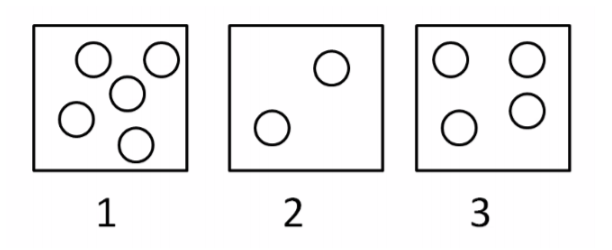
\includegraphics[scale=0.4]{img/ind_ball_i_bin.PNG}
\end{center}
In this example, you are able to count the number of balls in each bin, though. For example, there are 5 balls in bin 1, 2 balls in bin 2, and 4 balls in bin 3.

\subsubsection{Definitions}

\begin{definition}{Weak Composition}{}
    A weak composition of $n$ is a sequence of non-negative integers $a_1, a_2, ..., a_k$ so that $a_1 + a_2 + \dots + a_n = n$.
\end{definition}

\begin{definition}{Composition}{}
    A composition of $n$ is a sequence of positive integers $a_1, a_2, \dots, a_k$ so that $a_1 + a_2 + \dots + a_n = n$. These are sometimes known as \emph{strict compositions}.
\end{definition}

So, if we put $n$ balls into $k$ bins, letting $a_i$ be the number of balls in the $i$th bin, we get a (weak) composition of $n$ into $k$ parts. In this case:
\begin{itemize}
    \item If we allow the bins to be empty, we want weak compositions. 
    \item If we do not allow the bins to be empty (i.e. every bin must have at least one ball), we want strict compositions. 
\end{itemize}

\subsubsection{Stars and Bars}
In order to count compositions, we need a clever way of writing them. 
\begin{itemize}
    \item For each $i$, write $a_i$ many stars (\code{*}). 
    \item Separate these terms with a bar (\code{|}). In other words, where does one number start and where does the next one begin.
\end{itemize}
For example, 5 + 2 + 4 becomes:
\begin{verbatim}
    *****|**|****
\end{verbatim}
So, what happens if we write a weak composition of $n$ into $k$ parts in terms of stars and bars? We can get an arrangement with:
\begin{itemize}
    \item $n$ total stars.
    \item $k - 1$ total bars. 
\end{itemize}
And any such arrangement gives rise to binomial coefficients. 

\begin{theorem}{Number of Weak Compositions}{}
    For all positive integers $n$ and $k$, the number of weak compositions of $n$ into $k$ parts is:
    \[\binom{n + k - 1}{k - 1} = \binom{n + k - 1}{n}\]
\end{theorem}

What happens if we cannot allow bins to be empty? 
\begin{itemize}
    \item Then, we want compositions rather than weak compositions.
    \item We can relate the two. We have that $a_1, a_2, \dots, a_k$ is a composition of $n$ if and only if $a_1 - 1, a_2 - 1, \dots, a_k - 1$ is also a weak composition of $n - k$. 
    \item So, the number of composition of $n$ into $k$ parts equals the number of weak compositions of $n - k$ into $k$ parts, or $\binom{n - 1}{k - 1} = \binom{(n - k) + k - 1}{k - 1}$. 
\end{itemize}
We can also view this using stars and bars. Specifically, we need arrangements of $n$ stars and $k - 1$ bars where no two bars are adjacent and no bars are at the end. For example, these are invalid:
\begin{verbatim}
    |**|
    ***||**
\end{verbatim}
Consider the arrangement:
\begin{verbatim}
    *[ ]*[ ]*[ ]*[ ]*[ ]*[ ]*[ ]*[ ]
\end{verbatim}
Where \code{[ ]} represents possible locations for a bar. Then, we can select $k - 1$ locations from $n - 1$ options, so $\binom{n - 1}{k - 1}$ possiblities. 

\begin{corollary}{Number of Compositions}{}
    For all positive integers $n$ and $k$, the number of compositions (not weak compositions) of $n$ into $k$ parts is:
    \[\binom{n - 1}{k - 1}\]
\end{corollary}

What if we don't restrict the number of bins? Well, we need to consider a few things: 
\begin{itemize}
    \item Must only consider non-empty bins. Otherwise, we can just keep adding empty bins.
    \item Get the total number of compositions of $n$. 
    \item From the above argument, we have $n - 1$ positions for bars, and we can select any number of them.
    \item Well, this is simply the number of subsets of a set of size $n - 1$, or $2^{n - 1}$.
\end{itemize}

\begin{corollary}{Number of All Compositions}{}
    For all positive integers $n$, the number of all compositions (not weak compositions) of $n$ is:
    \[\sum_{k = 1}^{n} \binom{n - 1}{k - 1} = 2^{n - 1}\]
\end{corollary}

\subsection{Distinguishable Balls into Indistinguishable Bins: Set Partitions}
Consider balls labeled $1, 2, \dots, n$. We can tell which set of balls are in each bin. Here, we make use of set partitions to count these. 

\begin{definition}{Set Partition}{}
    A \textbf{set partition} of a set $S$ is a collection of non-empty subsets $S_1, S_2, \dots, S_k$ so that each element of $S$ is in exactly one of the $S_i$. 
\end{definition}

\begin{definition}{Stirling Numbers}{}
    The \textbf{stirling numbers of the second kind} are given by:
    \[S(n, k) = \text{ Number of partitions of $[n]$ into $k$ parts.}\]
\end{definition}
Note that $[n] = \{1, 2, 3, ..., n\}$.

\begin{theorem}{Stirling Numbers and Recurrence Relations}{}
    For all positive integers $k \leq n$ (and $n, k \geq 1$):
    \[S(n, k) = S(n - 1, k - 1) + k \cdot S(n - 1, k)\]
\end{theorem}
\begin{proof}
    A partition of $[n]$ into $k$ parts has either:
    \begin{itemize}
        \item $n$ is in a set by itself (i.e. $n$ is lone). In this case, removing $\{n\}$ will yield a partition of $[n - 1]$ into $k - 1$ parts. Thus, the number of such set partitions if $S(n - 1, k - 1)$. 
        \item $n$ is in a set with other elements. In this case, removing $n$ from whatever part it is in will yield a partition of $[n - 1]$ into $k$ parts. Of course, there are $S(n - 1, k)$ ways to choose this partition, and then $k$ ways to pick which part to insert $n$ into. Then, the total is simply $k \cdot S(n - 1, k)$. \qedhere 
    \end{itemize}
\end{proof}

\subsubsection{Example: Stirling Number}
What is $S(3, 2)$? 
\begin{itemize}
    \item The answer is \textbf{3}. There are 3 possible partitions that partition the set into two subsets:
    \begin{itemize}
        \item $\{1, 2\}, \{3\}$
        \item $\{1, 3\}, \{2\}$
        \item $\{2, 3\}, \{1\}$
    \end{itemize}
\end{itemize}


\subsubsection{Facts about Stirling Numbers}
\begin{itemize}
    \item $S(n, n) = 1$ (only partition is $\{1\}, \{2\}, \dots, \{n\}$).
    \item $S(n, 1) = 1$ (only partition is $\{1, 2, ..., n\}$).
    \item $S(0, 0) = 1$ (by definition).
    \item $S(n, n - 1) = \binom{n}{2}$.
    Any partition of $[n]$ into $n - 1$ parts must have $n - 2$ parts of size 1 and 1 part of size 2.
    \item $S(n, 2) = 2^{n - 1} - 1$. 
    Splitting $[n]$ into two subsets, one subset contains 1 plus some subset of $\{2, 3, ..., n\}$. The other contains the rest. We can use any subset of $\{2, 3, ..., n\}$ except for the entire thing (as then the other set will be empty). 
\end{itemize}

\begin{corollary}{}{}
    For all real numbers $x$ and all non-negative integers $n$:
    \[x^n = \sum_{k = 0}^n S(n, k) (x)_k\]
\end{corollary}

\begin{proof}
    We proceed by induction on $n$.
    \begin{itemize}
        \item[\mdiamond] \underline{Base Case:} Let $n = 0$. Then, $x^n = x^0 = 1$. Also, $S(0, 0)(x)_0 = 1 \cdot 1 = 1$.
        \item[\mdiamond] \underline{Inductive Step:} Assume that $x^{n - 1} = \sum_{k} S(n - 1, k) (x)_k$. Then: 
        \begin{equation*}
            \begin{aligned}
                \sum_{k = 1}^n S(n, k)(x)_k &= \sum_{k = 1}^n (S(n - 1, k - 1) + kS(m - 1, k))(x)_k \\ 
                &= \sum_{k = 1}^n S(n - 1, k - 1)(x)_k + \sum_{k = 1}^n kS(n - 1, k)(x)_k \\ 
                &= \sum_{k = 1}^{n - 1} S(n - 1, k)(x)_{k + 1} + \sum_{k = 1}^{n - 1} kS(n - 1, k)(x)_k \\ 
                &= \sum_{k = 1}^{n - 1} S(n - 1, k)((x)_{k + 1} + k(x)_k) \\ 
                &= \sum_{k = 1}^{n - 1} S(n - 1, k)(x)_{k}((x - k) + k) \\ 
                &= x\sum_{k = 1}^{n - 1} S(n - 1, k)(x)_k \\ 
                &= x^n
            \end{aligned}
        \end{equation*}
        This concludes the proof. \qedhere  
    \end{itemize}
\end{proof}

\subsubsection{Bell Numbers}
What about the \emph{total} number of set partitions of $[n]$? While there isn't a good formula, we can define one.

\begin{definition}{Bell Numbers}{}
    The bell number, $B(n)$, is the number of set partitions of a set of size $n$.
\end{definition}

\subsubsection{Example: Bell Numbers}
What is $B(3)$?

\begin{itemize}
    \item The answer is 5. The set partitions are:
    \begin{itemize}
        \item $\{1\} \{2\} \{3\}$
        \item $\{1, 2\} \{3\}$
        \item $\{1, 3\} \{2\}$
        \item $\{2, 3\} \{1\}$
        \item $\{1, 2, 3\}$
    \end{itemize}
\end{itemize}

\subsubsection{Bell Numbers in Terms of Stirling Numbers}
Because bell numbers are simply an enumeration of all possible set partitions:
\[B(n) = \sum_{k = 0}^n S(n, k)\]

But, what about a recursive definition? First, let's ask the question: what is the set containing $n$?
\begin{itemize}
    \item If size $k$, we know that there are $\binom{n - 1}{k - 1}$ possible sets.
    \item There are $B(n - k)$ ways to partition remaining elements. 
\end{itemize}
So, the recurrence relation is:
\[B(n) = \sum_{k = 1}^n \binom{n - 1}{k - 1}B(n - k)\]

\begin{theorem}{}{}
    For all non-negative integers $n$:
    \[B(n + 1) = \sum_{i = 0}^{n} \binom{n}{i} B(i)\]
\end{theorem}

\subsection{Indistinguishable Balls into Indistinguishable Bins: Integer Partitions}
Consider unlabeled balls into unlabeled boxes, like so:
\begin{center}
    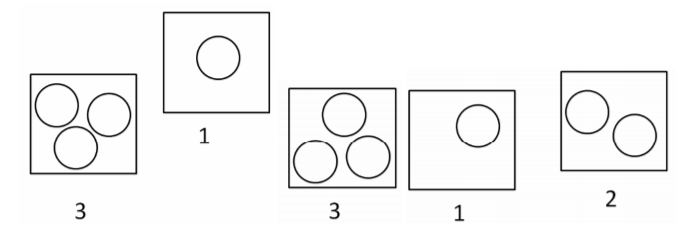
\includegraphics[scale=0.8]{img/i_ball_i_bin.PNG}
\end{center}

The question, then, is: \emph{what can we keep track of?}
\begin{itemize}
    \item Number of balls in each box.
\end{itemize}

\begin{definition}{Integer Partition}{}
    An \textbf{integer partition} of a positive number $n$ is a sequence of positive integers $a_1 \geq a_2 \geq \dots \geq a_k$ so that:
    \[a_1 + a_2 + \dots + a_k = n\]
    The $a_i$ are called the \textbf{parts} of the partition.  
\end{definition} 
\textbf{Remark:} 
\begin{itemize}
    \item Unlike compositions, this is an unordered collection of numbers. So, $3 + 3 + 2 + 1 + 1$ is the same as $3 + 2 + 3 + 1 + 1$. Because of this, we need to sort the numbers in decreasing order (hence the definition). 
    \item The integer partitions of $n$ correspond to the ways of putting $n$ unlabeled balls into nonempty boxes. 
\end{itemize}

\subsubsection{Example: Integer Partitions of 4}
\emph{How many integer partitions of 4 are there?}

\begin{itemize}
    \item There are 5 partitions. 
    \begin{itemize}
        \item 4 = 4
        \item 3 + 1 = 4
        \item 2 + 2 = 4
        \item 2 + 1 + 1 = 4
        \item 1 + 1 + 1 + 1 = 4
    \end{itemize}
\end{itemize}

\subsubsection{Partition Function}
There is no clean formula. However, we can come up with a definition.
\begin{definition}{Partition Function}{}
    $p(n)$ is the number of integer partitions of $n$. $p_{k}(n)$ is the number of partitions of $n$ into exactly $k$ parts. 
\end{definition}

\begin{theorem}{}{}
    $p_{k}(n)$ is the number of partitions of $n$ with the largest part of size $k$.
\end{theorem}

\subsubsection{Ferrers Diagram}
A Ferrers Diagram is a way to visualize partitions. In particular, we note that the $i$th row has $a_i$ squares. For instance, consider the Ferrers Diagram:
\begin{center}
    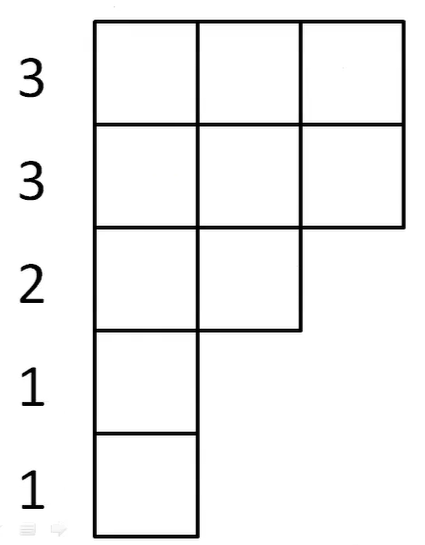
\includegraphics[scale=0.3]{img/ferrer.PNG}
\end{center}
This corresponds to the partition $3 + 3 + 2 + 1 + 1 = 10$. 

\bigskip 

There are some properties of Ferrers Diagrams to know.
\begin{itemize}
    \item Total number of squares equals total size of partitions (i.e. it adds up to $n$).
    \item No gaps. For any square in the diagram, the square above and the square to the left are also in the diagram (unless this would go over the edge). 
    \item One-to-one correspondence between partitions and Ferrers diagrams. 
\end{itemize}

\subsubsection{Conjugates}
Given a Ferrers diagram, we can come up with what is known as a \textbf{conjugate} Ferrers diagram. This is done by \emph{flipping the rows and columns}.

\bigskip 

Consider the example that we used above. Then:
\begin{center}
    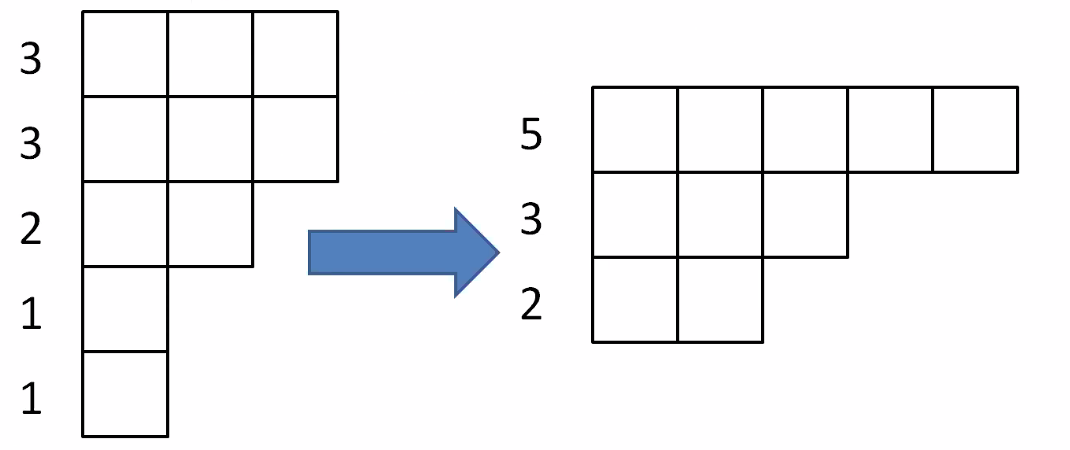
\includegraphics[scale=0.3]{img/conj.PNG}
\end{center}
So, the conjugate of $3 + 3 + 2 + 1 + 1$ is $5 + 3 + 2$. 

\bigskip 

There are some properties of conjugates to keep in mind.
\begin{itemize}
    \item The size of a partition and its conjugate are the same. In other words, each have the same number of squares.
    \item The conjugate of the conjugate of a partition is the original partition.
    \item The number of parts in a partition equals the size of the largeest part of its conjugate.
\end{itemize}

\subsubsection{Self-Conjugate Partitions}
\begin{definition}{Self-Conjugate}{}
    A partition is called \emph{self-conjugate} if it is the same as its conjugate. 
\end{definition}
Here is an example of a self-conjugate partition:
\begin{center}
    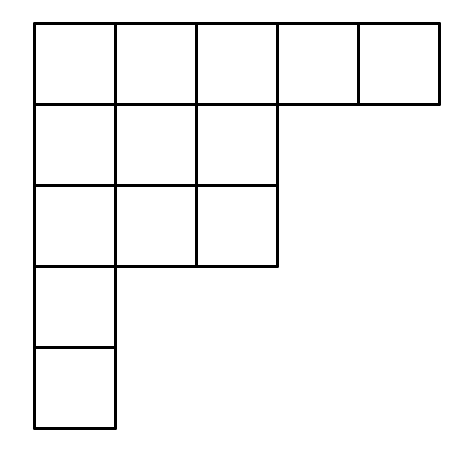
\includegraphics[scale=0.3]{img/self_c.PNG}
\end{center}
The squares in the Ferrers diagram for any self-conjugate partition can be decomposed into Ls. In the example shown below, we have $9 + 3 + 1$. 
\begin{center}
    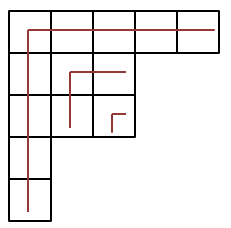
\includegraphics[scale=0.8]{img/self_c_L.PNG}
\end{center}
 
\begin{itemize}
    \item Each L has an odd number of squares (self-conjugate).
    \item Each L has fewer squares than the outer ones. In other words, they must nest. 
\end{itemize}
As a result, we have the following theorem: 
\begin{theorem}{}{}
    The number of self-conjugate partitions of $n$ is the same as the number of partitions of $n$ in to distinct, odd parts. 
\end{theorem}

\subsection{Summary}
\begin{center}
    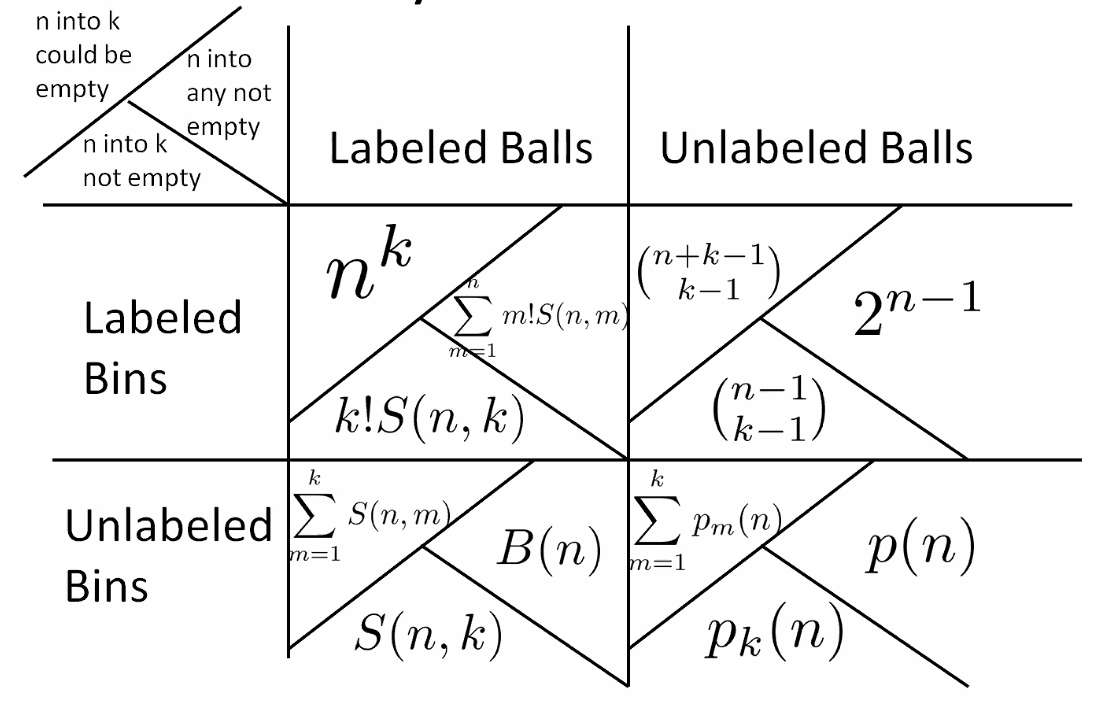
\includegraphics[scale=0.6]{img/summary_ballbin.PNG}
\end{center}






% --------------------------------------------------------- %
%                   NEW SECTION                             %
% --------------------------------------------------------- %
\newpage 
\section{Binomial Theorem and Related Identities}
Recall the identities that we have found already to be useful:
\[\sum_{k = 0}^n \binom{n}{k} = 2^n\]
\[\sum_{k = 0}^n (-1)^k \binom{n}{k} = 0 \qquad \text{For } n > 0\]
These can all be generalized using the binomial theorem.

\subsection{The Binomial Theorem}
\begin{theorem}{The Binomial Theorem}{}
    For all non-negative integers $n$:
    \[(x + y)^n = \sum_{k = 0}^n \binom{n}{k} x^k y^{n - k}\]
\end{theorem}

\begin{proof}
    We can prove the binomial theorem by induction on $n$. 

    \begin{itemize}
        \item \underline{Base Case:} Let $n = 1$. Then:
        \[(x + y)^1 = x + y = \binom{1}{0}x^1 y^0 + \binom{1}{1} x^0 y^1\]

        \item \underline{Inductive Step:} Suppose that the binomial theorem is true for $n$. We want to show that this is true for $n + 1$. So, by doing some algebra:
        \begin{equation*}
            \begin{aligned}
                (x + y)^{n + 1} &= (x + y)(x + y)^n \\ 
                    &= (x + y)\sum_{k = 0}^n \binom{n}{k} x^k y^{n - k} \\ 
                    &= \sum_{k = 0}^n \binom{n}{k} x^{k + 1} y^{n - k} + \sum_{k = 0}^n \binom{n}{k} x^k y^{n - k + 1} \\ 
                    &= \sum_{k = 1}^{n + 1} \binom{n}{k - 1} x^k y^{n - k + 1} + \sum_{k = 0}^n \binom{n}{k} x^k y^{n - k + 1} \\ 
                    &= \sum_{k = 0}^{n + 1} \left(\binom{n}{k - 1} + \binom{n}{k}\right) x^k y^{n - k + 1} \\ 
                    &= \sum_{k = 0}^{n + 1} \binom{n + 1}{k} x^k y^{n - k + 1}
            \end{aligned}
        \end{equation*}
        This concludes the proof. \qedhere
    \end{itemize}
\end{proof}

\subsection{Applications}
There are some important theorems from the textbook. 
\begin{theorem}{}{}
    For all positive integers $n$, the alternating sum of binomial coefficients $\binom{n}{k}$ is zero. In other words:
    \[\sum_{k = 0}^n (-1)^k \binom{n}{k} = 0\]
\end{theorem}
\begin{proof}
    Let $x = -1$ and $y = 1$. Substitute this into the binomial theorem to get the result. 
\end{proof}

\begin{theorem}{}{}
    For all non-negative integers $n$, the identity holds:
    \[2^n = \sum_{k = 0}^n \binom{n}{k}\]
\end{theorem}
\begin{proof}
    Let $x = y = 1$. Substitute this into the binomial theorem to get the result. 
\end{proof}

\begin{theorem}{}{}
    For all non-negative integers $n$, the identity holds:
    \[n2^{n - 1} = \sum_{i = 0}^{n} i \binom{n}{i}\]
\end{theorem}
\begin{proof}
    Take the derivative of both sides of the binomial theorem with respect to $x$ to get $n(x + y)^{n - 1} = \sum_{i = 0}^{n} i\binom{n}{i}x^{i - 1}y^{n - i}$. Then, let $x = y = 1$. 
\end{proof}

\begin{theorem}{}{}
    For all non-negative integers $n$ and $k$, the identity holds:
    \[\binom{n}{k} + \binom{n}{k + 1} = \binom{n + 1}{k + 1}\]
\end{theorem}

\begin{theorem}{}{}
    For all non-negative integers $k$ and $n$:
    \[\binom{k}{k} + \binom{k + 1}{k} + \binom{k + 2}{k} + \dots + \binom{n}{k} = \binom{n + 1}{k + 1}\]
\end{theorem}

\begin{theorem}{}{}
    For positive integers $n$ and $k$:
    \[\binom{n}{k} = \sum_{m = k}^n \binom{m - 1}{k - 1}\]
\end{theorem}

\begin{theorem}{Vandermonde's Identity}{}
    For all positive integers $n$, $m$, and $k$:
    \[\binom{n + m}{k} = \sum_{i = 0}^k \binom{n}{i} \binom{m}{k - i}\]
\end{theorem}

\begin{definition}{Multinomial Coefficients}{}
    Let $n = \sum_{i = 1}^k a_i$, where $n$ and $a_1$, $a_2$, \dots, $a_k$ are non-negative integers. We define:
    \[\binom{n}{a_1,a_2,\dots,a_k} = \frac{n!}{a_{1}! a_{2}! \dots a_{k}!}\]
\end{definition}

\begin{theorem}{Multinomial Theorem}{}
    For all non-negative integers $n$ and $k$, the following equality holds.
    \[(x_1 + x_2 + \dots + x_k)^n = \sum_{a_1,a_2,\dots,a_k} \binom{n}{a_1,a_2,\dots,a_k} x_{1}^{a_1} x_{2}^{a_2} \dots x_{k}^{a_k}\]
    Here, the sum is taken over all $k$-tuples of non-negative integers $a_1$, $a_2$, \dots, $a_k$ such that $n = \sum_{i = 1}^k a_i$. 
\end{theorem}

\begin{theorem}{}{}
    For all non-negative integers $n$ and $a_1$, $a_2$, \dots, $a_k$ such that $n = \sum_{i = 1}^n a_i$, the following equality holds:
    \[\binom{n}{a_1,a_2,\dots,a_k} = \binom{n}{a_1}\dots\binom{n - a_1 - \dots - a_i}{a_{i + 1}}\dots\binom{n - a_1 - \dots - a_{k - 1}}{a_k}\]
\end{theorem}

\begin{definition}{Generalized Binomial Coefficient}{}
    Let $m$ be any \underline{real} number and let $k$ be a non-negative integer. Then, $\binom{m}{0} = 1$. Additionally, for $k > 0$:
    \[\binom{m}{k} = \frac{m(m - 1)\dots(m - k + 1)}{k!}\]
\end{definition}

\begin{theorem}{Generalized Binomial Theorem}{}
    Let $m$ be any \underline{real} number. Then:
    \[(1 + x)^m = \sum_{n \geq 0} \binom{m}{n} x^n = 1 + mx + m(m - 1)\frac{x^2}{2} + \dots + (m)_k \frac{x^k}{k!}\]
    Where the sum is taken over all non-negative integers $n$.
\end{theorem}








% --------------------------------------------------------- %
%                   NEW SECTION                             %
% --------------------------------------------------------- %
\newpage 
\section{Permutations and Cycle Structures}
Now, we will talk more about permutations and, in particular, cycle structures.

\subsection{Permutations}
\begin{definition}{Permutation}{}
    A \textbf{permutation} of $[n]$ is a list of the numbers from 1 to $n$ with each number appearing exactly once. Looking at the positions of each number, this is equivalent to a bijection $\pi: [n] \to [n]$.  
\end{definition}

\subsubsection{Example: Number of Permutations}
\emph{How many permutations of $[n]$ are there?}
\begin{itemize}
    \item The answer is $\mathbf{n!}$. At the beginning, we have $n$ choices. Once we choose one number, we are left with $n - 1$ choices. After removing that number, we have $n - 2$ choices. Keep on doing this, we will eventually have $(n)(n - 1)(n - 2) \dots (2)(1)$ choices, or $n!$. 
    \item Another way of seeing it is: There are $n$ options for $\pi(1)$, then $n - 1$ options for $\pi(2)$, and so on until we have 1 option left for $\pi(n)$.
\end{itemize}

\subsection{Repeated Application}
Suppose that you have a permutation $\pi$ of $[n]$ and some integer $1 \leq m \leq n$. What happens when you repeatedly apply $\pi$ to $m$? That is:
\[m \to \pi(m) \to \pi(\pi(m)) \to \dots\]
\begin{lemma}{}{}
    Let $\pi: [n] \to [n]$ be a permutation and let $x \in [n]$. Then, there exists a positive integer $1 \leq i \leq n$ so that $\pi^{i}(x) = x$. 
\end{lemma}

\subsection{Cycles}
So, not only does $m$ repeat itself, it is actually the \emph{first} element of this sequence to repeat itself. In particular, if $k$ is the smallest integer so that $\pi^{k}(m) = m$, we have that $m$, $\pi(m)$, $\pi^{2}(m)$, \dots, $\pi^{k - 1}(m)$ are all distinct and $\pi^{k}(m) = m$.

\bigskip 

From there, the sequence repeats itself. This sequence $m$, $\pi(m)$, $\pi^{2}(m)$, \dots, $\pi^{k - 1}(m)$ is known as a \emph{cycle}. So, given any permutation $\pi$ of $[n]$, we can partition $[n]$ into cycles. 

\bigskip 

For instance, consider \code{7146352}. This permutation has two cycles.
\begin{center}
    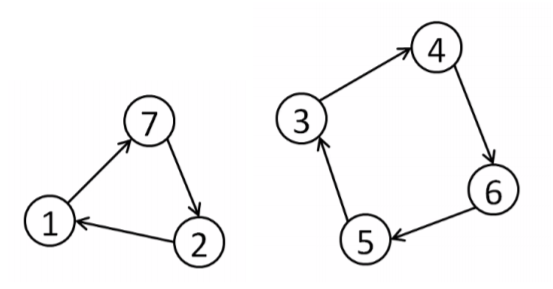
\includegraphics[scale=0.5]{img/ex_cycle.PNG}
\end{center}

\bigskip 

We can also look at the permutation \code{14253}. This permutation also has two cycles:
\begin{center}
    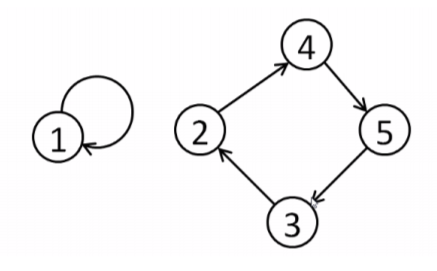
\includegraphics[scale=0.5]{img/ex_cycle_2.PNG}
\end{center}

\subsection{Cycle Representation}
As every element is part of some cycle, if you can specify what each cycle is, you can specify the permutation. 

\subsubsection{Example: Cycle Representation}
\code{7146352} is the permutation with cycles:
\begin{itemize}
    \item $1 \to 7 \to 2 \to 1$.
    \item $3 \to 4 \to 6 \to 5 \to 3$.
\end{itemize}
Any permutation of $[7]$ with these cycles must be \code{7146352}.

\subsubsection{Cycle Notation}
To write this more conveniently:
\begin{itemize}
    \item Write each cycle by writing the elements in order contained within parentheses.
    \item Write the permutation by writing each cycle in it. 
\end{itemize}

\subsubsection{Non-Uniqueness}
One issue with this representation is that there are multiple ways to write the same permutation. This is because of two things:
\begin{itemize}
    \item A cycle can start at any position. For example:
    \[(172) = (721) = (217)\]
    
    \item Cycles can be listed in any order:
    \[(172)(3465) = (3465)(172)\]
\end{itemize}

\subsubsection{Canonical Cycle Notation}
One way to fix this is to remove this freedom by specifying an order. One way to do this is using \emph{canonical cycle notation}. 

\begin{definition}{Canonical Cycle Notation}{}
    For any given permutation of $[n]$, we can write it out in Canonical Cycle Notation. In this form, each cycle will be written with its largest element first, and cycles will be written in increasing order of their first elements. 
\end{definition}

\subsubsection{Example: CCN of 58237614}
Consider the permutation, \code{58237614}. 
\begin{itemize}
    \item Cycles: (157), (2843), (6).
    \item In CCN, we write these cycles as: (715), (8432), (6).
    \item So, in CCN, the whole permutation is written as: (6)(715)(8432).
\end{itemize}

\subsection{Permutations with Particular Cycle Structure}

\begin{theorem}{Permutations with Particular Cycle Structures}{}
    Let $a_1$, $a_2$, \dots, $a_n$ be non-negative integers so that the equality $\sum_{i = 1}^n i \cdot a_i = n$ holds. Then, the number of $n$-permutations with $a_i$ cycles of length $i$ where $i \in [n]$ is:
    \[\frac{n!}{a_{1}!a_{2}!\dots a_{n}!1^{a_1}2^{a_2}\dots n^{a_n}}\]
\end{theorem}

\subsubsection{Example: Counting}
How many permutations of $[9]$ have three cycles of length 1 and two cycles of length 3?
\begin{itemize}
    \item Idea: Writing in cycle notation and this permutation must be:
    \[(x_1)(x_2)(x_3)(x_4 x_5 x_6)(x_7 x_8 x_9)\]
    Where $x_1$, $x_2$, \dots, $x_9$ are 1, 2, \dots, 9 in some order. Then, there are $9!$ ways to assign each $x_i$ a different elements of $[9]$. Is that the answer? Nope.

    \bigskip 
    
    This is because we are overcounting. This is not canonical cycle notation because the same permutation can be written in multiple ways. Instead, we consider the following:
    \begin{itemize}
        \item We can rearrange the three 1-cycle in $3! = 6$ ways.
        \item Each of the \emph{three} 1-cycles can start with any 1 element.
        \item We can rearrange the two 3-cycle in $2! = 2$ ways. 
        \item Each of the \emph{two} 3-cycles can start with any of their 3 elements. 
    \end{itemize}
    So, each such permutation can be written in $3!1^3 2!3^2$ many ways. Thus, the final answer is:
    \[\frac{9!}{3!1^3 2!3^2} = 3360\] 
\end{itemize}

\subsection{Stirling Numbers}
\begin{definition}{Stirling Number of the First Kind}{}
    The number of permutations of $[n]$ with $k$ cycles is called a \emph{unsigned Stirling number of the first kind} and is given by:
    \[c(n, k) = \text{Number of Permutations of } [n] \text{ with } k \text{ Cycles.}\]
    The number $s(n, k) = (-1)^{n - k} c(n, k)$ is called a \emph{Stirling number of the first kind}. 
\end{definition}
\textbf{Remark:} There are some properties of Stirling numbers to keep in mind.
\begin{itemize}
    \item $c(n, n) = 1$ (Must have $n$ 1-cycle).
    \item $c(n, 1) = (n - 1)!$ (One $n$-cycle).
    \item $c(n, n - 1) = \frac{n(n - 1)}{2}$ (One 2-cycle and $n - 2$ 1-cycles).
    \item $c(n, 2) = \sum_{k = 1}^{n} \frac{n!}{2k(n - k)}$
\end{itemize}

\begin{theorem}{}{}
    Let $n$ and $k$ be positive integers such that $n \geq k$. Then:
    \[c(n, k) = c(n - 1, k - 1) + (n - 1)c(n - 1, k)\]
\end{theorem}

\begin{proof}
    This can be broken down into two cases. Suppose we have $n$ people and $k$ tables arranged in a circle. Additionally, suppose $c(n, k)$ is the total number of distinct seating arrangements of $n$ people into $k$ tables. 
    \begin{itemize}
        \item \underline{Case 1:} Suppose the $n$th person sits at his or her own table. Then, we have $n - 1$ people and $k - 1$ tables left. In this sense, it follows that there are $c(n - 1, k - 1)$ ways to arrange the $n - 1$ remaining people with the $k - 1$ remaining tables. 
        \item \underline{Case 2:} Now suppose that all but the $n$th person has been seated at every table; in particular, every table has at least one person. This amounts to $c(n - 1, k)$. Of course, we need to seat the $n$th person somewhere! So, how many distinct ways can we seat the $n$th person? Well, we can put the $n$th person next to one of the other people; since there are $n - 1$ remaining people, we can put the $n$th person next to someone to get a unique seating arrangement. Thus, there are $(n - 1)c(n - 1, k)$ ways to place our $n$th person.
    \end{itemize}
    All possible arrangements of $n$ people into $k$ tables either have person $n$ seated by themselves or amongst the others, so it follows that:
    \[c(n, k) = c(n - 1, k - 1) + (n - 1)c(n - 1, k)\]
    Where $n \geq 1$ and $k \geq 1$. \qedhere 
\end{proof}

\begin{lemma}{}{}
    Let $n$ be a fixed positive integer. Then:
    \[\sum_{k = 0}^n c(n, k) x^k = x(x + 1)\dots (x + n - 1)\]
\end{lemma}

\subsection{Study of Individual Cycle Sizes}
\begin{lemma}{}{}
    Let $i \in [n]$. Then, for all $k \in [n]$, there are exactly $(n - 1)!$ permutations of length of length $n$ in which the cycle containing $i$ is of length $k$. 
\end{lemma}
\begin{proof}
    The proof by direct counting is intuitive:
    \begin{itemize}
        \item $n - 1$ options for $\pi(n)$ (anything but $n$).
        \item $n - 2$ options for $\pi^{2}(n)$ (anything but $n$ or $\pi(n)$).
        \item $n - 3$ options for $\pi^{3}(n)$ (anything but $n$ or $\pi(n)$ or $\pi^{2}(n)$).
        \item \dots
        \item $n - k + 1$ options for $\pi^{k - 1}(n)$.
        \item 1 option for $\pi^{k}(n) = n$. 
        \item $(n - k)!$ options for the permutation of the other $n - k$ elements.
        \item Multiply together to get $(n - 1)!$ total elements.  \qedhere 
    \end{itemize}
\end{proof}
There is another proof we can use, and this uses canonical cycle notation:
\begin{proof}
    When you write the permutation in canonical cycle notation, the cycle containing $n$ is exactly everything listed from the appearance of $n$ onward. So, $n$ is in a cycle of length $k$ if and only if $n$ is written $k$th from last. There are $(n - 1)!$ ways to arrange the other $n - 1$ elements into the other $n - 1$ spots.
\end{proof}

\subsection{EVEN and ODD}
Now, we will talk about the notion of \emph{even} and \emph{odd} cycles, or cycles that have only cycles of even and odd lengths, respectively. 

\begin{lemma}{}{}
    For all positive integers $m$, the equality $ODD(2m) = EVEN(2m)$ holds.
\end{lemma}

For the above lemma, there is a nice bijection that you can use to prove this. In particular, the algorithm behind this is as follows.
\begin{itemize}
    \item Work from the last cycle to the first cycle. 
    \item If the last element of the last cycle is \emph{smaller} than the first element of the next-to-last cycle, then move that element from the last cycle to the end of the next-to-last cycle. 
    \item \emph{Otherwise}, move the last element from the last cycle into its own singleton between said cycle and the one before it. 
    \item Move on to the next \emph{untouched} cycle. 
\end{itemize}

\begin{theorem}{}{}
    For all positive integers $m$:
    \[ODD(2m) = EVEN(2m) = (2m - 1)^2  (2m - 3)^2 (2m - 5)^2 \dots 3^2 1^2\]
\end{theorem}

\begin{theorem}{}{}
    For all positive integers $m$:
    \[ODD(2m + 1) = (2m + 1) \cdot ODD(2m) = (2m + 1) (2m - 1)^2 (2m - 3)^2 (2m - 5)^2 \dots 3^2 1^2\]
    Additionally:
    \[EVEN(2m + 1) = 0\]
\end{theorem}








% --------------------------------------------------------- %
%                   NEW SECTION                             %
% --------------------------------------------------------- %
\newpage 
\section{Inclusion-Exclusion}
Now, we will briefly discuss inclusion-exclusion.

\subsection{Addition Rule}
Recall that if $S$ and $T$ are \underline{disjoint} sets, then:
\[|S \cup T| = |S| + |T|\]

\subsubsection{Question: Student Majors}
\emph{Suppose that registered for this class, we have 100 math majors, 15 computer science majors, 10 economics majors, and no one else. How many students are there total?}
\begin{itemize}
    \item Impossible to determine. What if there are double majors? If there are double majors, they will be counted in more than one category. 
\end{itemize}

\subsubsection{Question: Student Majors}
\emph{Suppose we have 15 computer science majors and 10 economics major, but 2 of them are CS-Economics double major. How many do we have in total?}
\begin{itemize}
    \item There are $15 - 2 = 13$ pure computer science majors, $10 - 2 = 8$ pure economics majors, and 2 double majors. These are all disjoint sets of people. So, there are $13 + 8 + 2 = 23$ people in total. 
\end{itemize}

\subsection{Generalized Addition Rule}
\begin{theorem}{}{}
    For any sets $S$ and $T$ we have that:
    \[|S \cup T| = |S| + |T| - |S \cap T|\]
\end{theorem}
\textbf{Remark:} If $|S \cap T| = 0$, then this recovers the usual addition rule. 

\subsection{The Theorem}
\begin{theorem}{Generalized Inclusion-Exclusion}{}
    Given any finite sets $S_1, S_2, \dots, S_n$, we have that:
    \[|S_1 \cup S_2 \cup \dots \cup S_n| = \sum_{k = 1}^n (-1)^{k - 1} \sum_{1 \leq i_1 \leq i_2 \leq \dots \leq i_k \leq n} |S_{i_{1}} \cap S_{i_{2}} \cap \dots \cap S_{i_{k}}|\]
    More clearly, we have:
    \[\left| \bigcup_{i = 1}^n S_i \right| = \sum_{i = 1}^n |S_i| - \sum_{i < j} |S_i \cap S_j| + \sum_{i < j < k} |S_i \cap S_j \cap S_k| - \dots + (-1)^{n - 1} |S_1 \cap \dots S_n|\]
\end{theorem}

\subsubsection{For Two Sets}
Inclusion-exclusion for two sets $A$ and $B$ is simply:
\[|A \cup B| = |A| + |B| - |A \cap B|\]

\subsubsection{For Three Sets}
Inclusion-exclusion for three sets $A$, $B$, and $C$ is simply:
\[|A \cup B \cup C| = |A| + |B| + |C| - |A \cap B| - |B \cap C| - |A \cap C| + |A \cap B \cap C|\]

\subsubsection{For Four Sets}
Inclusion-exclusion for four sets $A$, $B$, $C$, and $D$ is simply:
\begin{equation*}
    \begin{aligned}
        |A \cup B \cup C \cup D| &= |A| + |B| + |C| + |D| \\ 
            &- |A \cap B| - |A \cap C| - |A \cap D| - |B \cap C| - |B \cap D| - |C \cap D| \\ 
            &+ |A \cap B \cap C| + |A \cap B \cap D| + |A \cap C \cap D| + |B \cap C \cap D| \\
            &- |A \cap B \cap C \cap D|
    \end{aligned}
\end{equation*}


\subsection{Applications}
Here, we discuss some applications of Inclusion-Exclusion.

\subsubsection{Stirling Numbers}
Recall that the number of way to put $n$ labeled balls into $k$ labeled, non-empty boxes is $k!S(n, k)$ (First, pick the set partition, then pick which part goes into which box). Recall that this is the same as the number of \emph{surjections} from a set of size $[n]$ to a size $[k]$. If we can count this, then we can compute Stirling numbers. 

\bigskip 

To motivate this, consider the question: \emph{How many surjections are there $[n] \to [3]$?}
\begin{itemize}
    \item There are $3^n$ total functions, but not all are surjections. Which are we missing?
    \begin{itemize}
        \item Functions that don't have 1 in their range.
        \begin{itemize}
            \item How many functions $[n] \to [3]$ don't have 1 in their image? These are functions $[n] \to \{2, 3\}$, or simply $2^n$ such functions. The similar argument can be made for the other cases. 
        \end{itemize}
        \item Functions that don't have 2 in their range.
        \item Functions that don't have 3 in their range. 
    \end{itemize}
    \item Combining these, we have $3^n - 2^n - 2^n - 2^n$. However, we aren't done. These removed sets overlap, so we need to use inclusion-exclusion. Let's do this more formally. 
    \begin{itemize}
        \item Let $A_1$, $A_2$, and $A_3$ denote the sets of functions missing 1, 2, and 3 respectively. Then, we want $3^n - |A_1 \cup A_2 \cup A_3|$.
        \item Using Inclusion-Exclusion:
        \[\boxed{3^n - |A_1| - |A_2| - |A_3| + |A_1 \cap A_2| + |A_2 \cap A_3| + |A_1 \cap A_3| - |A_1 \cap A_2 \cap A_3|}\]
        \item What is $|A_1 \cap A_2|$? The functions taking value neither 1 nor 2. In other words, this is only the function that assigns 3 to everything. This applies to the other pairwise intersections.
        \item What about $|A_1 \cap A_2 \cap A_3|$? These are the functions not taking values 1, 2, or 3. There are no functions that have this criteria. 
        \item So, the answer is simply:
        \[3^n - 2^n - 2^n - 2^n + 1 + 1 + 1 = \boxed{3^n - 3 \cdot 2^n + 3}\]
        So, therefore:
        \[\boxed{S(n, 3) = \frac{3^{n - 1}}{2} + 2^{n - 1} + \frac{1}{2}}\]
    \end{itemize}
\end{itemize}
Generalizing this, $S(n, k)$ represents the number of partitions of $[n]$ into $k$ parts. If we label the parts $1, 2, \dots, k$ (can be done in $k!$ ways), we get a surjection $[n] \to [k]$. So:
\[\{\text{Number of Surjections } [n] \to [k]\} = k!S(n, k)\]
How many surjections are there? Well, counting all functions is easy. A function fail to be a surjection if and only if some value fails to be in the image. Let $S$ be the set of all functions $[n] \to [k]$. Let $A_i$ be the set of functions $[n] \to [k]$ with $i$ not in the image. So, the number of surjections is simply:
\begin{equation*}
    \begin{aligned}
        \text{Num. Surjections} &= |S| - |A_1 \cup A_2 \cup \dots \cup A_k| \\ 
            &= k^n - |A_1 \cup A_2 \cup \dots \cup A_k| \\ 
            &= k^n - \sum_{m = 1}^{k} (-1)^{m - 1} \sum_{1 \leq i_1 < i_2 < \dots < i_m \leq k} |A_{i_1} \cap A_{i_2} \cap \dots \cap A_{i_m}|
    \end{aligned}
\end{equation*}
But since $A_{i_1} \cap A_{i_2} \cap \dots \cap A_{i_m}$ is the set of functions from $[n]$ to $[k]$ such that $i_1, i_2, \dots, i_m$ do not appear in the image, we have that: 
\[|A_{i_1} \cap A_{i_2} \cap \dots \cap A_{i_m}| = \text{Num. Functions From } [n] \to [k - \{i_1, i_2, \dots, i_m\}]\]
Thus:
\begin{equation*}
    \begin{aligned}
        \text{Num. Surjective Functions} &= k^n - \sum_{m = 1}^{k} (-1)^{m - 1} \sum_{1 \leq i_1 < i_2 < \dots < i_m \leq k} |A_{i_1} \cap A_{i_2} (k - m)^n \\ 
            &= k^n - \sum_{m = 1}^{k} (-1)^{m - 1} (k - m)^n \binom{k}{m} \\ 
            &= k^n + \sum_{m = 1}^{k} (-1)^m (k - m)^n \binom{k}{m} \\ 
            &= \sum_{m = 0}^{k} (-1)^m (k - m)^n \binom{k}{m}
    \end{aligned}
\end{equation*}
Putting this together, we have:
\[k!S(n, k) = \sum_{m = 0}^{k} (-1)^m (k - m)^n \binom{k}{m} \implies S(n, k) = \sum_{m = 0}^{k} (-1)^m \frac{(k - m)^n}{k!}\]
Which leads to the following theorem: 
\begin{theorem}{Stirling Numbers of the Second Kind}{}
    For all positive integers $n$ and $k$, the following equality holds:
    \[S(n, k) = \frac{1}{k!} \sum_{i = 0}^k (-1)^i \binom{k}{i} (k - i)^n = \sum_{i = 0}^k (-1)^i \frac{(k - i)^n}{i!(k - i)!}\]
\end{theorem}

\subsubsection{Derangements}
We want to count the number of permutations $\pi: [n] \to [n]$ satisfying a bunch of conditions:
\begin{itemize}
    \item $\pi(1) \neq 1$.
    \item $\pi(2) \neq 2$. 
    \item \dots
    \item $\pi(n) \neq n$. 
\end{itemize}
Each condition is relatively easy to deal with individually, but many at once is hard. Combining these, the conditions are hard. But, if we negate them, it becomes easier. In other words, we don't want any of the following:
\begin{itemize}
    \item $\pi(1) = 1$.
    \item $\pi(2) = 2$. 
    \item \dots
    \item $\pi(n) = n$. 
\end{itemize}
Letting $A_i$ be the permutations $\pi$ of $[n]$ with $\pi(i) = i$, we let:
\[D_n = n! - |A_1 \cup A_2 \cup \dots \cup A_n|\]
Then, using inclusion-exclusion:
\[|A_1 \cup A_2 \cup \dots \cup A_n| = \sum_{k = 1}^n (-1)^{k - 1} \sum_{1 \leq i_1 < i_2 < \dots < i_k \leq n} |A_{i_{1}} \cap A_{i_{2}} \cap \dots \cap A_{i_{k}}|\]
We first ask: how big is $|A_{i_1} \cap A_{i_2} \cap \dots \cap A_{i_k}|$? This is the set of permutations of $[n]$ so that:
\begin{itemize}
    \item $\pi(i_1) = i_1$.
    \item $\pi(i_2) = i_2$.
    \item \dots
    \item $\pi(i_k) = i_k$.
\end{itemize}
These $k$ values are fixed, and we can use any permutation on the other $n - k$ elements, so the total size of $(n - k)!$. Thus:
\begin{equation*}
    \begin{aligned}
        D_n &= n! - \sum_{k = 1}^n (-1)^{k - 1} \sum_{1 \leq i_1 < i_2 < \dots < i_k \leq n} |A_{i_{1}} \cap A_{i_{2}} \cap \dots \cap A_{i_{k}}| \\ 
            &= n! - \sum_{k = 1}^n (-1)^{k - 1} \sum_{1 \leq i_1 < i_2 < \dots < i_k \leq n} (n - k)! \\ 
            &= n! - \sum_{k = 1}^n (-1)^{k - 1} (n - k)! \binom{n}{k} \\ 
            &= n! - \sum_{k = 1}^n (-1)^{k - 1} \frac{n!}{k} \\ 
            &= n! \left(1 - \sum_{k = 1}^{n} (-1)^{k - 1} \frac{1}{k!}\right)
    \end{aligned}
\end{equation*}
This gives us the following definition: 
\begin{definition}{Derangements}{}
    A derangement is a permutation with no 1-cycles. This is denoted by $D_n$, or the number of derangements of $[n]$ with no 1-cycles, and can be found using the formula:
    \[D_n = n! - \sum_{k = 1}^n (-1)^{k - 1} \frac{n!}{k!}\]
\end{definition}









% --------------------------------------------------------- %
%                   NEW SECTION                             %
% --------------------------------------------------------- %
\newpage 
\section{Generating Functions}
In order to study some interesting sequence of numbers, $a_0, a_1, a_2, \dots$, we can turn these numbers into a single function $f(x) = a_0 + a_{1}x + a_{2}x^2 + \dots$ and study $f(x)$. 

\bigskip 

The point is that because the elements of the sequence are just the coefficients of $x$ in this power series, $f(x)$ encodes the sequence that we are interested in.

\begin{definition}{Ordinary Generating Functions}{}
    Let $\{f_n\}_{n \geq 0}$ be a sequence of real numbers. Then, the formal power series $F(x) = \sum_{n \geq 0}^{\infty} f_n x^n$ is called the \emph{ordinary generating function} of the sequence $\{f_n\}_{n \geq 0}$. 
\end{definition}

\subsection{What is a Generating Function?}
We can interpret a generating function $F(x)$ in two ways: 
\begin{itemize}
    \item As an \textbf{actual function} of a (real or complex) variable $x$, this should converge for $x$ in some range. 
    \item A \textbf{formal power series}, namely a set of symbols that can be manipulated in the same way real function could, but that can't necessarily be evaluated anywhere. 
\end{itemize}


\subsection{Purpose}
Why is this a good idea? 
\begin{enumerate}
    \item The function $f$ can encode the sequence $\{a_i\}$ within a single function. 
    \item Complicated combinatorical properties of the sequence $\{a_i\}$ can often be encoded as algebraic or analytic properties of $f(x)$. 
    \item This often lets us reduce solving complicated problems to basic algebra.  
\end{enumerate}


\subsection{Application: Recurrence Relations}
A \emph{recurrence relation} is a way of defining a sequence of numbers by giving a formula for each element in terms of the previous ones. 

\bigskip 

To find the closed form of a recurrence relation, we can make use of generating functions.

\subsubsection{Example 1: Basic Recurrence}
To better demonstrate this, consider the recurrence relation\footnote{The following steps can be applied to exponential generating functions.}:
\[a_n = \begin{cases}
    2 & n = 0 \\
    4 & n = 1 \\  
    3a_{n - 1} - 2 & \text{Otherwise}
\end{cases}\]
To find the closed form for this recurrence relation: 
\begin{enumerate}[(1)]
    \item Define the generating function $F(x) = \sum_{n = 0}^{\infty} a_n x^n = a_0 + a_1 x + a_2 x^2 + \dots$. 
    \item Account for the base case(s). These will usually take up $a_0$, $a_1$, and so on. In this case:
    \[F(x) = \boxed{a_0 + a_1 x} + a_2 x^2 + a_3 x^3 + \dots = \boxed{2 + 4x} + a_2 x^2 + \dots\]
    \item For the remaining $a_i$ terms, substitute the generating function in its place. Then, expand it out. 
    \begin{equation*}
        \begin{aligned}
            F(x) &= 2 + 4x + \boxed{\sum_{n = 0}^{\infty} a_{n + 2} x^{n + 2}} \\ 
                &= 2 + 4x + \boxed{\sum_{n = 2}^{\infty} a_{n} x^{n}} \\ 
                &= 2 + 4x + \boxed{\sum_{n = 2}^{\infty} (3a_{n - 1} - 2) x^{n}} \\ 
                &= 2 + 4x + \boxed{\sum_{n = 2}^{\infty} 3a_{n - 1} x^n - \sum_{n = 2}^{\infty} 2x^n}
        \end{aligned}
    \end{equation*}
    \item Change all instances of the summation into $F(x)$ defined in step 1 or another known generating function. This will usually involve shifting the summations. 
    \begin{equation*}
        \begin{aligned}
            F(x) &= 2 + 4x + \sum_{n = 2}^{\infty} 3a_{n - 1} x^n - \sum_{n = 2}^{\infty} 2x^n = 2 + 4x + \sum_{n = 1}^{\infty} 3a_{n} x^{n + 1} - 2 \sum_{n = 2}^{\infty} x^n \\ 
                &= 2 + 4x + 3x \sum_{n = 1}^{\infty} a_{n} x^{n} - 2 \sum_{n = 0}^{\infty} x^{n + 2} = 2 + 4x + 3x \left(\sum_{n = 0}^{\infty} a_{n} x^{n} - a_0 x^0\right) - 2x^2 \sum_{n = 0}^{\infty} x^n \\ 
                &= 2 + 4x + 3x \left(\boxed{\sum_{n = 0}^{\infty} a_{n} x^{n}} - 2\right) - \boxed{2x^2 \sum_{n = 0}^{\infty} x^n}\\ 
                &= 2 + 4x + 3x \left(\boxed{F(x)} - 2\right) - \boxed{\frac{2x^2}{1 - x}} \\ 
                &= 2 + 4x + 3xF(x) - 6x - \frac{2x^2}{1 - x}
        \end{aligned}
    \end{equation*}
    \item Isolate $F(x)$ so that you get a rational function. 
    
    \bigskip 

    Since we have:
    \[F(x) = 2 + 4x + 3xF(x) - 6x - \frac{2x^2}{1 - x}\]
    It follows that: 
    \[F(x) - 3xF(x) = 2 + 4x - 6x - \frac{2x^2}{1 - x} \iff F(x) = \frac{2 - 2x - \frac{2x^2}{1 - x}}{1 - 3x} = \boxed{\frac{2 - 4x}{(1 - x)(1 - 3x)}}\]
    This gives us the \textbf{closed form} of the generating function. 

    \item Use partial fraction decomposition on $F(x)$. 
    
    \bigskip 
    
    In particular, using partial fraction decomposition, we have:
    \[F(x) = \frac{A}{(1 - x)} + \frac{B}{(1 - 3x)}\]
    So:
    \[\frac{A}{(1 - x)} + \frac{B}{(1 - 3x)} = \frac{A(1 - 3x) + B(1 - x)}{(1 - x)(1 - 3x)}\]
    We want:
    \[2 - 4x = A(1 - 3x) + B(1 - x) = (A + b) - (3A + B)x\]
    Solving for $A$ and $B$, we have:
    \[A = B = 1\]
    And, as a result, we have that:
    \[F(x) = \frac{1}{1 - x} + \frac{1}{1 - 3x}\]

    \item Find a new generating function that encodes this. Then, find the explicit formula from the coefficient of the generating function. 
    
    \bigskip 
    
    We know how to encode each of the terms of the generating function. That is:
    \[\frac{1}{1 - x} = \sum_{n = 0}^{\infty} x^n \qquad \frac{1}{1 - 3x} = \sum_{n = 0}^{\infty} (3x)^n\]
    So, our generating function is:
    \[F(x) = \sum_{n = 0}^{\infty} x^n + \sum_{n = 0}^{\infty} (3x)^n\] 
    Following up on this, we have:
    \begin{equation*}
        \begin{aligned}
            F(x) &= \sum_{n = 0}^{\infty} x^n + \sum_{n = 0}^{\infty} (3x)^n \\ 
                &= \sum_{n = 0}^{\infty} x^n + \sum_{n = 0}^{\infty} 3^n x^n \\ 
                &= \sum_{n = 0}^{\infty} \boxed{(1 + 3^n)} x^n
        \end{aligned}
    \end{equation*}
    So, our explicit formula is:
    \[a_n = 1 + 3^n\]
\end{enumerate}

\subsubsection{Example 2: Fibonacci}
Consider the Fibonacci sequence defined by:
\[a_n = \begin{cases}
    1 & n = 0 \\ 
    1 & n = 1 \\ 
    a_{n - 1} + a_{n - 2} & \text{Otherwise}
\end{cases}\]

\begin{enumerate}[(1)]
    \item Define the generating function $F(x) = \sum_{n = 0}^{\infty} a_{n} x^{n}$. 
    \item Account for the base case(s). 
    \[F(x) = \boxed{a_0 + a_1 x^1} + a_2 x^2 + a_3 x^3 + \dots = \boxed{1 + x} + a_2 x^2 + a_3 x^3 + \dots\]
    
    \item For the remaining $a_i$ terms, substitute the generating function in its place. 
    \begin{equation*}
        \begin{aligned}
            F(x) &= 1 + x + \boxed{\sum_{n = 2}^{\infty} (a_{n - 1} + a_{n - 2}) x^n} \\ 
                &= 1 + x + \boxed{\sum_{n = 2}^{\infty} a_{n - 1} x^n + \sum_{n = 2}^{\infty} a_{n - 2} x^n}
        \end{aligned}
    \end{equation*}

    \item Change all instances of the summation into $F(x)$ defined in step 1 or another known generating function. This will usually involve shifting the summations.
    \begin{equation*}
        \begin{aligned}
            F(x) &= 1 + x + \sum_{n = 2}^{\infty} a_{n - 1} x^n + \sum_{n = 2}^{\infty} x^n \\ 
                &= 1 + x + \sum_{n = 0}^{\infty} a_{n + 1} x^{n + 2} + \sum_{n = 0}^{\infty} a_{n} x^{n + 2} \\ 
                &= 1 + x + x \sum_{n = 0}^{\infty} a_{n + 1} x^{n + 1} + x^2 \sum_{n = 0}^{\infty} a_n x^n \\ 
                &= 1 + x + x \left(\sum_{n = 0}^{\infty} a_n x^n - a_0 x^0\right) + x^2 \sum_{n = 0}^{\infty} a_n x^n \\ 
                &= 1 + x + x \left(\sum_{n = 0}^{\infty} a_n x^n - 1\right) + x^2 \sum_{n = 0}^{\infty} a_n x^n \\ 
                &= 1 + x + x \left(F(x) - 1\right) + x^2 F(x)
        \end{aligned}
    \end{equation*}

    \item Isolate $F(x)$ so that you get a rational function. 
    
    \bigskip 

    Since we have:
    \[F(x) = 1 + x + x(F(x) - 1) + x^2 F(x) \iff F(x) = 1 + xF(x) + x^2 F(x)\]
    It follows that:
    \[F(x) - xF(x) - x^2 F(x) = 1 \iff (1 - x - x^2)F(x) = 1 \iff F(x) = \boxed{\frac{1}{1 - x - x^2}}\]

    \item Use partial fraction decomposition on $F(x)$. 
    
    \bigskip 

    This function isn't exactly super nice when it comes to partial fraction decomposition. That being said, we know that:
    \[1 - x - x^2 = \left(x - \frac{-1 + \sqrt{5}}{2}\right)\left(x - \frac{-1 - \sqrt{5}}{2}\right)\]
    So, it follows that:
    \begin{equation*}
        \begin{aligned}
            F(x) &= \frac{A}{\left(x - \frac{-1 + \sqrt{5}}{2}\right)} + \frac{B}{\left(x - \frac{-1 - \sqrt{5}}{2}\right)} \\ 
                &= \frac{1}{\sqrt{5}} \frac{1}{\left(x - \frac{-1 + \sqrt{5}}{2}\right)} - \frac{1}{5} \frac{1}{\left(x - \frac{-1 - \sqrt{5}}{2}\right)} \\ 
                &= \frac{1}{\sqrt{5}} \left(\frac{1}{\left(x - \frac{-1 + \sqrt{5}}{2}\right)} - \frac{1}{\left(x - \frac{-1 - \sqrt{5}}{2}\right)}\right)
        \end{aligned}
    \end{equation*}

    \item Find a new generating function that encodes this. Then, find the explicit formula from the coefficient of the generating function. 
    
    \bigskip 

    Let $\alpha = \frac{-1 + \sqrt{5}}{2}$ and $\beta = \frac{-1 - \sqrt{5}}{2}$. Then:
    \begin{equation*}
        \begin{aligned}
            F(x) &= \frac{1}{\sqrt{5}} \left(\frac{1}{x - \alpha} - \frac{1}{x - \beta}\right) \\ 
                &= \frac{1}{\sqrt{5}} \left(\frac{\frac{1}{\alpha}}{\frac{1}{\alpha}x - 1} - \frac{\frac{1}{\beta}}{\frac{1}{\beta}x - 1}\right) \\ 
                &= \frac{1}{\sqrt{5}} \left(\frac{\frac{1}{\beta}}{1 - \frac{1}{\beta}x} - \frac{\frac{1}{\alpha}}{1 - \frac{1}{\alpha}x}\right) \\ 
                &= \frac{1}{\sqrt{5}} \left(\sum_{n = 0}^{\infty} \left(\frac{1}{\beta}\right)^{n + 1} x^n - \sum_{n = 0}^{\infty} \left(\frac{1}{\alpha}\right)^{n + 1} x^n\right) \\ 
                &= \sum_{n = 0}^{\infty} \frac{1}{\sqrt{5}} \left(\left(\frac{1}{\beta}\right)^{n + 1} - \left(\frac{1}{\alpha}\right)^{n + 1}\right) x^n
        \end{aligned}
    \end{equation*}
    So, our explicit formula is:
    \begin{equation*}
        \begin{aligned}
            a_n &= \frac{1}{\sqrt{5}} \left(\left(\frac{1}{\beta}\right)^{n + 1} - \left(\frac{1}{\alpha}\right)^{n + 1}\right) \\ 
                &= \frac{1}{\sqrt{5}} \left[\left(\frac{2}{-1 - \sqrt{5}}\right)^{n + 1} - \left(\frac{2}{-1 + \sqrt{5}}\right)^{n + 1}\right] \\ 
                &= \frac{1}{\sqrt{5}} \left[\left(\frac{1 - \sqrt{5}}{2}\right)^{n + 1} - \left(\frac{1 + \sqrt{5}}{2}\right)^{n + 1}\right]
        \end{aligned}
    \end{equation*}
\end{enumerate}

\subsection{Tools and Operations}
\textbf{Remark:} There are several basic tools and operations that we can use to evaluate generating functions.
\begin{itemize}
    \item If two generating functions are the same, the coefficients are the same. That is, if $\sum_{n \geq 0}^{\infty} a_n x^n = \sum_{n \geq 0}^{\infty} b_n x^n$ for all $n$, then $a_n = b_n$ for all $n$. 
    
    \item Geometric Series:
    \[\frac{1}{1 - cx} = \sum_{n \geq 0}^{\infty} (cx)^n = \sum_{n \geq 0}^{\infty} c^n x^n\]

    \item Sums of Generating Functions: 
    \[\sum_{n \geq 0}^{\infty} a_n x^n + \sum_{n \geq 0}^{\infty} b_n x^n = \sum_{n \geq 0}^{\infty} (a_n + b_n) x^n\]

    \item Shifts: If $F(x) = \sum_{n \geq 0}^{\infty} a_n x^n$, then
    \[xF(x) = \sum_{n \geq 0}^{\infty} a_n x^{n + 1} = \sum_{n > 0}^{\infty} a_{n - 1} x^n\]

    \item Scaling: We can multiply a generating function by a constant, which scales every term in the associated sequence by the same constant. For example, given the generating function:
    \[F(x) = \sum_{n \geq 0}^{\infty} a_n x^n = a_0 x^0 + a_1 x^1 + a_2 x^2 + \dots\]
    Multiplying this generating function by a constant $c$ gives:
    \[cF(x) = c\sum_{n \geq 0}^{\infty} a_n x^n = ca_0 x^0 + ca_1 x^1 + ca_2 x^2 + \dots\]
    
    \item Differentiation: We can also take the derivative of a generating function, which in turn will take the derivative of every term in the associated sequence. For example, given the generating function:
    \[F(x) = \sum_{n \geq 0}^{\infty} a_n x^n = a_0 x^0 + a_1 x^1 + a_2 x^2 + \dots\]
    Taking the derivative gives us:
    \begin{equation*}
        \begin{aligned}
            \frac{d}{dx} F(x) &= \frac{d}{dx} \sum_{n \geq 0}^{\infty} a_n x^n \\ 
                &= \sum_{n \geq 1}^{\infty} n a_n x^{n - 1} \\
                &= \sum_{n \geq 0}^{\infty} (n + 1)a_{n + 1}x^n \\
                &= \frac{d}{dx} a_0 x^0 + \frac{d}{dx} a_1 x^1 + \frac{d}{dx} a_2 x^2 + \dots \\
                &= a_1 + 2a_2 x + 3a_3 x^2 + \dots
        \end{aligned}
    \end{equation*}
\end{itemize}

\subsection{Basic Generating Functions}
There are several basic generating functions to know. More are listed in the appendix.
\begin{itemize}
    \item For the sequence 1, 1, 1, \dots.
    \[F(x) = \sum_{n \geq 0}^{\infty} x^n = \frac{1}{1 - x} = 1 + x + x^2 + x^3 + x^4 + \dots\]
    
    \item For the sequence 1, -1, 1, -1, \dots.
    \[F(x) = \sum_{n \geq 0}^{\infty} (-x)^n = \sum_{n \geq 0}^{\infty} (-1)^n x^n = \frac{1}{1 - (-x)} = \frac{1}{1 + x} = 1 - x + x^2 - x^3 + x^4 - \dots\]
    
    \item For the sequence 1, 2, 3, 4, \dots.
    \[F(x) = \left(\sum_{n \geq 0}^{\infty} x^n\right)^2 = \frac{1}{(1 - x)^2} = 1 + 2x + 3x^2 + 4x^3 + \dots\]
    
    \item For the sequence 1, -2, 3, -4, \dots.
    \[F(x) = \left(\sum_{n \geq 0}^{\infty} (-x)^n\right)^2 = \frac{1}{(1 - (-x))^2} = \frac{1}{(1 + x)^2} = 1 - 2x + 3x^2 - 4x^3 + 5x^4 - \dots\]

    \item For the sequence 1, 0, 1, 0, \dots.
    \[F(x) = \sum_{n \geq 0}^{\infty} (x^2)^n = \sum_{n = 0}^{\infty} x^{2n} = \frac{1}{1 - x^2} = 1 + x^2 + x^4 + x^6 + \dots\]
\end{itemize}
More of these are listed in the appendix. 

\subsection{Products of Generating Functions}
\begin{lemma}{Products of Generating Functions}{}
    Let $\{a_n\}_{n \geq 0}$ and $\{b_n\}_{n \geq 0}$ be two sequences and let $A(x) = \sum_{n \geq 0}^{\infty} a_n x^n$ and $B(x) = \sum_{n \geq 0}^{\infty} b_n x^n$ be their respective generating functions. Then, we can define $c_n = \sum_{i = 0}^n a_i b_{n - i}$ and let $C(x) = \sum_{n \geq 0}^{\infty} c_n x^n$. Then:
    \[A(x)B(x) = C(x)\]
    Here, we can say that the coefficients of $x^n$ in $A(x)B(x)$ is $c_n = \sum_{i = 0}^n a_i b_{n - i}$.  
\end{lemma} 

\begin{theorem}{The Product Formula}{}
    Suppose you have objects of type $A$ and objects of type $B$. Each has a size which is a non-negative integer, and there are $a_n$ objects of type $A$ of size $n$ and $b_m$ objects of type $B$ of size $m$. 
    
    \bigskip 
    
    Then, $c_k$ is the number of ways to find a pair of an object of type $A$ and an object of type $B$ where the sum of the sizes is $k$. 
\end{theorem}


\subsection{Compositions of Generating Functions}
\begin{definition}{Composition of Generating Functions}{}
    Let $F(x) = \sum_{n \geq 0}^{\infty} f_n x^n$ be a formal power series and let $G$ be a formal power series with constant term 0. Then, we can define:
    \[F(G(x)) = \sum_{n \geq 0}^{\infty} f_n (G(x))^n = f_0 + f_1 G(x) + f_2 G(x)^2 + \dots\] 
\end{definition} 

\begin{theorem}{The Compositional Formula}{}
    Let $a_n$ be the number of ways to build a certain structure on an $n$-element set and assume that $a_0 = 0$. Let $b_n$ be the number of ways to build a second structure on an $n$-element set and let $b_0 = 1$. Let $g_n$ be the number of ways to split the set $[n]$ into an unspecified number of non-empty intervals, build a structure of the first kind on each of these intervals, and then build a structure of the second kind on the set of the intervals. Let $g_0 = 1$. Then, let $A(x)$, $B(x)$, and $G(x)$ be the generating functions of the sequences $\{a_n\}$, $\{b_n\}$, $\{g_n\}$. Then:
    \[G(x) = B(A(x))\]
\end{theorem}

\subsection{Catalan Numbers}
To motivate this, consider the question: \emph{How many ways can you produce $n$ matching pairs of parentheses?}

\bigskip 

For $n = 2$, we can have:
\begin{itemize}
    \item \code{()()}
    \item \code{(())}
\end{itemize}
The idea is that we must have $n$ \code{(} and $n$ \code{)}. In this sense, we could say that there are $\binom{2n}{n}$ ways to arrange these parentheses. However, not all of these work. For instance, the following are invalid (for $n = 2$):
\begin{itemize}
    \item \code{))((}
    \item \code{)()(}
\end{itemize}
The idea is that we cannot, at any point, have more closing parentheses than opening parentheses. 

\bigskip 

One way to count this is to image an $n \times n$ graph, something like:
\begin{center}
    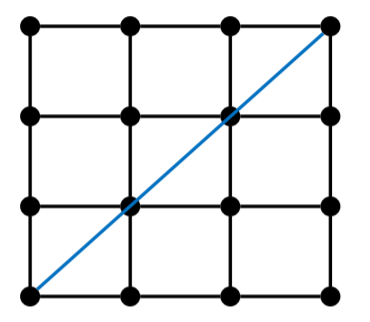
\includegraphics[scale=0.6]{img/graph_cat.PNG}
\end{center}
Here, we can make steps of either $(0, 1)$ or $(1, 0)$, and the graph starts at $(0, 0)$ and ends at $(n, n)$. So, for a parenthesis pattern, we can create a path where we can keep track of the number of left parentheses and the number of right parentheses:
\[(\text{Num. Left Paren.}, \text{Num. Right Paren.})\]
So, how many such paths are there? 
\begin{definition}{Catalan Numbers}{}
    The $n$th Catalan number $C_n$ is the number of up-left lattice paths from $(0, 0)$ to $(n, n)$ that stay on or above the line $y = x$.
\end{definition}
To start counting, we need to consider which parentheses \code{(} matches with. In this sense, we can say that it matches with the $k$th \code{)} for some $k$. 
\[\underbrace{(...)}_{k - 1 \text{ pairs}} \qquad \underbrace{...}_{n - k \text{ pairs}}\]
So:
\begin{itemize}
    \item There are $C_{k - 1}$ ways to match the first group.
    \item There are $C_{n - k}$ ways to match the second group. 
\end{itemize}
And, as a result, we have:
\[C_n = \sum_{k = 1}^{n} C_{k - 1} C_{n - k}\]
Using generating functions, we arrive at the following conclusion:
\begin{definition}{Catalan Number Function}{}
    Recursively, the $n$th Catalan number is defined by:
    \[C_n = \sum_{k = 1}^n C_{k - 1}C_{n - k}\]
    Using generating functions, we can define a closed form version by:
    \[C_n = \frac{1}{n + 1} \binom{2n}{n}\]
\end{definition}








% --------------------------------------------------------- %
%                   NEW SECTION                             %
% --------------------------------------------------------- %
\newpage 
\section{Exponential Generating Functions}
Like ordinary generating functions, this is a way to associate sequence of numbers that we're interested in studying to some power series.

\bigskip 

The only difference is that, for expoenntial generating functions, we have:
\[\{a_n\} \longleftrightarrow \sum_{n = 0}^{\infty} a_n \frac{x^n}{n!}\]
Whereas for ordinary generating functions:
\[\{a_n\} \longleftrightarrow \sum_{n = 0}^{\infty} a_n x^n\]

\subsection{Comparison Between Ordinary and Exponential Generating Functions}
\begin{center}
    \begin{tabular}{c|c}
        \textbf{Ordinary} & \textbf{Exponential} \\ 
        \hline 
        $F(x) = \sum_{n = 0}^{\infty} a_n x^n$ & $F(x) = \sum_{n = 0}^{\infty} a_n \frac{x^n}{n!}$ \\ 
        $a_n = 1$ and $F(x) = \frac{1}{1 - x}$ & $a_n = 1$ and $F(x) = e^x$ \\ 
        $a_n = n$ and $F(x) = \frac{x}{(1 - x)^n}$ & $a_n = n$ and $F(x) = xe^x$ \\ 
        $xF(x) = \sum_{n = 0}^{\infty} a_n x^{n + 1} = \sum_{n > 0}^{\infty} a_{n - 1} x^n$ & $\sum_{n = 0}^{\infty} a_{n + 1} \frac{x^n}{n!} = F'(x)$ \\ 
        Converges only if $a_n$ grows at most exponentially. & Converges more generally.
    \end{tabular}
\end{center}

\subsection{Multiplication of Exponential Generating Function}
Multiplication of ordinary generating functions is important, but it is also different compared to ordinary generating function. 

\bigskip 

Let's suppose we have two generating functions:
\[A(x) = \sum_{n = 0}^{\infty} a_n \frac{x^n}{n!}\]
\[B(x) = \sum_{n = 0}^{\infty} b_n \frac{x^n}{n!}\]
\[C(x) = A(x)B(x) = \sum_{n = 0}^{\infty} c_n \frac{x^n}{n!}\]
Where:
\[c_n = \sum_{k = 0}^{n} \binom{n}{k} a_k b_{n - k}\]

\subsection{Combinatorial Interpretation of Multiplication}
\begin{itemize}
    \item Define an $A$-structure to be a thing so that there are $a_n$ $A$-structures on a set of size $n$. 
    \item Define a $B$-structure to be a thing so that there are $b_n$ $B$-structures on a set of size $n$. 
    \item Ordinary generating function multiplication talks about the number of ways to find an $A$-structure and a $B$-structure of total size $n$. 
    \item Exponential generating function multiplication has $c_n$ be the number of ways to partition $[n]$ into two sets and put an $A$-structure on one and a $B$-structure on the other. 
    \item If the $A$-structure has size $k$, then there are $\binom{n}{k}$ ways to partition $[n]$ into $a_k$ $A$-structures and $b_{n - k}$ $B$-structures.
\end{itemize}

\subsection{Composition of Generating Functions}
Let's suppose we have two generating functions:
\[A(x) = \sum_{n = 0}^{\infty} a_n \frac{x^n}{n!}\]
\[B(x) = \sum_{n = 0}^{\infty} b_n \frac{x^n}{n!}\]
\[B(A(x)) = \sum_{n = 0}^{\infty} b_n \frac{A(x)^n}{n!}\]
So, the $\frac{x^n}{n!}$ coefficient is:
\begin{itemize}
    \item $b_1$ times the number of partitions of $[n]$ into one part with an $A$-structure; plus
    \item $b_2$ times the number of partitions of $[n]$ into two parts with an $A$-structure on each; plus 
    \item \dots 
\end{itemize}

Summing these all together, the $\frac{x^n}{n!}$ coefficient of $B(A(x))$ counts the number of ways to partition $[n]$ into subsets, put an $A$-structure on each subset, and put a $B$-structure on the collection of subsets.

\subsection{Applications}
Some applications of exponential generating functions are as follows. 

\subsubsection{Permutations}
A permutation of $[n]$ is equivalent to partitioning $[n]$ into subsets and then arranging each subset into a cycle. 

\bigskip 

The $A$-structure is a cycle. There are $(k - 1)!$ cycles on a $k$-element subset so $a_k = (k - 1)!$. Then:
\[A(x) = \sum_{k \geq 1}^{\infty} (k - 1)! \frac{x^k}{k!} = \sum_{k \geq 1}^{\infty} \frac{x^k}{k} = \log\left(\frac{1}{1 - x}\right)\]

\subsubsection{Stirling Numbers}
What if we count permutations of $[n]$ weighted by $y^{\text{Number of Cycles}}$?
\begin{itemize}
    \item The $A$-structure is a cycle. 
    \item The $B$-structure has $b_n = y^n$. Here, $B(x) = \sum_{n = 0}^{\infty} x^n \frac{y^n}{n!} = e^{xy}$. 
\end{itemize}
The generating function is:
\[B(A(x)) = e^{y\log(\frac{1}{1 - x})} = \left(\frac{1}{1 - x}\right)^y\]
The $y^k \frac{x^n}{n!}$-coefficient is the number of permutations of $[n]$ with $k$ cycles.  

\bigskip 

This leads the following theorem.
\begin{theorem}{Unsigned Stirling Numbers of the First Kind}{}
    \[\sum_{n, k = 0}^{\infty} c(n, k) \frac{x^n}{n!} y^k = \left(\frac{1}{1 - x}\right)^y\]
\end{theorem}

\subsubsection{At Least Subsets}
How many ways can $[n]$ be partitioned into an even number of subsets of size at least 2?
\begin{itemize}
    \item The $A$-structure is the subset of size at least 2. Here, $a_n = 1$ if $n \geq 0$ and 0 otherwise. So, $A(x) = e^x - 1 - x$. 
    \item The $B$-structure (which is supposed to tell you what you are supposed to do once you have these subsets) is an even number of subsets. Here, $b_n = 1$ is $n$ is even and 0 otherwise. Our generating function is $B(x) = \cosh(x) = \frac{e^x + e^{-x}}{2}$. 
\end{itemize}
The generating function is the composition:
\[\cosh(e^x - 1 - x)\]

\subsubsection{Derangements}
What about derangements of $[n]$? 
\begin{itemize}
    \item A-structure is a cycle of length \textbf{not} 1.
    \begin{itemize}
        \item $a_n = (n - 1)!$ unless $n = 1$, in which case $a_n = 0$. The generating function is:
        \[A(x) = \log\left(\frac{1}{1 - x}\right) - x\]

        \item B-structure is any partition. 
        \[B(x) = e^x\]
    \end{itemize}
\end{itemize}
Generating function is:
\[B(A(x)) = e^{\log\left(\frac{1}{1 - x}\right) - x} = \frac{e^{-x}}{1 - x}\]
If we wanted a permutations without 2-cycles, we would get:
\[\frac{e^{-\frac{x^2}{2}}}{1 - x}\]
Here, we got this by setting $A(x)$ equal to the same generating function as above, but with $a_n = 0$ for $n = 2$ instead of $n = 1$.

\subsubsection{Permutations with Even/Odd Length Cycles}
What about permutations with only cycles of even length or only odd length? 
\begin{itemize}
    \item A-structure is a cycle of appropriate length.
    \begin{itemize}
        \item $a_n = (n - 1)!$ if $n$ is even, 0 otherwise.
        \item Generating function is:
        \[A(x) = \sum_{n \text{ even}} \frac{x^n}{n}\]
    \end{itemize}
\end{itemize}
How do you restrict a generating function to only the even terms? Let $f(x) = \sum_n a_n x^n$ be a generating function. Then:
\[f(-x) = \sum_{n} (-1)^n a_n x^n\]
Then:
\[f(x) + f(-x) = \sum_n (1 + (-1)^n) a_n x^n = 2 \sum_{n \text{ even}} a_n x^n\]
And so: 
\[\frac{f(x) + f(-x)}{2} = \sum_{n \text{ even}} a_n x^n\]
Similarly, for odd terms: 
\[\frac{f(x) - f(-x)}{2} = \sum_{n \text{ odd}} a_n x^n\]
Thus, the generating function for the A-structure of cycles of even length is:
\[\sum_{n \text{ even}} \frac{x^n}{n} = \frac{\log\left(\frac{1}{1 - x}\right) + \log\left(\frac{1}{1 + x}\right)}{2} = \log\left(\frac{1}{\sqrt{1 - x^2}}\right)\]
It follows that the generating function for permutations with even length cycles is:
\[\boxed{\sum_{n = 0}^{\infty} EVEN(n) \frac{x^n}{n!} = e^{\log\left(\frac{1}{\sqrt{1 - x^2}}\right)} = \frac{1}{\sqrt{1 - x^2}}}\]
The generating function for the A-structure of cycles of odd length is: 
\[\sum_{n \text{ odd}} \frac{x^n}{n} = \frac{\log\left(\frac{1}{1 - x}\right) - \log\left(\frac{1}{1 + x}\right)}{2} = \log\left(\sqrt{\frac{1 + x}{1 - x}}\right)\]
Thus, the generating function for permutations with odd length cycles is:
\[\boxed{\sum_{n = 0}^{\infty} ODD(n) \frac{x^n}{n!} = e^{\log\left(\sqrt{\frac{1 + x}{1 - x}}\right)} = \sqrt{\frac{1 + x}{1 - x}}}\]

\subsection{Other Generating Functions}
\begin{itemize}
    \item Stirling Numbers of the Second Kind
    \[\sum_{n, k = 0}^{\infty} S(n, k) \frac{x^n}{n!} y^k = e^{y(e^x - 1)}\]
    \item Bell Numbers 
    \[\sum_{n = 0}^{\infty} B(n) \frac{x^n}{n!} = e^{e^x - 1}\]
    \item Derangements 
    \[\sum_{n = 0}^{\infty} D_n \frac{x^n}{n!} = \frac{e^{-x}}{1 - x}\]
\end{itemize}







% --------------------------------------------------------- %
%                   NEW SECTION                             %
% --------------------------------------------------------- %
\newpage 
\section{Pattern Avoidance in Permutations}
\begin{itemize}
    \item Patterns in Permutations 
    \item Some Basic Counting Results 
    \item Asymptotic Results 
\end{itemize}

\subsection{The Stack}
A \textbf{stack} is an object that stores numbers. You can push more numbers onto it, or you can pop the most recently pushed number off. 

\subsubsection{Stack-Sortable Permutations}
\begin{definition}{}{}
    A permutation $\pi$ of $[n]$ is stack-sortable if there is a series of operations that involve $1, 2, \dots, n$ being pushed into a stack in $\pi$ order and popped off the stack in sorted order. 
\end{definition}

For example, \code{312} is stack-sortable:
\begin{verbatim}
    Operation           Stack           Popped 
    ---------------------------------------------
    push(3)             [3]             []
    push(1)             [3, 1]          []
    pop()               [3]             [1]
    push(2)             [3, 2]          [1]
    pop()               [3]             [1, 2]
    pop()               []              [1, 2, 3]
\end{verbatim}

Another example we can look at is \code{632154}, which is stack-sortable:
\begin{verbatim}
    Operation           Stack           Popped 
    ---------------------------------------------
    push(6)             [6]             []
    push(3)             [6, 3]          []
    push(2)             [6, 3, 2]       []
    push(1)             [6, 3, 2, 1]    []
    pop()               [6, 3, 2]       [1]
    pop()               [6, 3]          [1, 2]
    pop()               [6]             [1, 2, 3]
    push(5)             [6, 5]          [1, 2, 3]
    push(4)             [6, 5, 4]       [1, 2, 3]
    pop()               [6, 5]          [1, 2, 3, 4]
    pop()               [6]             [1, 2, 3, 4, 5]
    pop()               []              [1, 2, 3, 4, 5, 6]
\end{verbatim}

Yet another example we can look at is \code{231}, which is \textbf{not} stack-sortable:
\begin{verbatim}
    Operation           Stack           Popped 
    ---------------------------------------------
    push(2)             [2]             []
    push(3)             [2, 3]          []
    push(1)             [2, 3, 1]       []
    pop()               [2, 3]          [1]
    pop()               [2]             [1, 3]
\end{verbatim}

\subsubsection{Sortability}
Which permutations are stack-sortable?
\begin{itemize}
    \item We can never stack larger values on top of smaller values.
    \item Must pop $i$ before any $j > i$ shows up.
    \item This is a problem if some $k < i$ shows up after $j$. 
\end{itemize}

\subsubsection{Classification}
\begin{theorem}{}{}
    A permutation is stack-sortable unless there are entries $k < i < j$ so that $i$ occurs before $j$ which occurs before $k$. 
\end{theorem}

\begin{proof}
    If such $i, j, k$ exists, it is not stack-sortable. But, if no such $i, j, k$ exist, we can use the following algorithm.
    \begin{itemize}
        \item Pop the stack when the next element to be added is bigger than the one on top or if there are no more elements. 
    \end{itemize}
    Here, we note that the elements in the stack are always in decreasing sorted order. This is because we only add elements smaller than the current top element.
    \begin{itemize}
        \item Pop $i$ when $j > i$ is about to be pushed. 
        \item No $k < i$ remains to be pushed. 
        \item No $k < i$ is below $i$ on the stack.
    \end{itemize}
    Therefore, the elements are popped in sorted order.
\end{proof}

So, $\pi$ is stack-sortable unless there are three entries $i$ that comes before $j$ that comes before $k$ with $k < i < j$. Equivalently, unless there are $x < y < z$ with $\pi(z) < \pi(x) < \pi(y)$. Or, three entries where the second smallest comes before the biggest comes before the smallest. 

\subsection{Patterns}
\begin{definition}{}{}
    Given two permutations $\pi$ of $[n]$ and $\rho$ of $[m]$, we say that there is a copy of $\rho$ in $\pi$ if there are $1 \leq x_1 < x_2 < \dots < x_m \leq n$ so that $\pi(x_1), \pi(x_2), \dots, \pi(x_m)$ have the \textbf{same relative orders} as $\rho(1), \rho(2), \dots, \rho(m)$. 
\end{definition}
For example, a permutation $\pi$ is stack-sortable if and only if it doesn't have a copy of \code{231}. 

\bigskip 

\textbf{Remark:} Suppose we have a permutation \code{42513}. Let's say we select three random elements \code{2}, \code{5} and \code{3}. What we are saying is what the sorted relative order is. We know that \code{132} means that the smallest number goes first (\code{1}), then the biggest (\code{3}), and then the next biggest (\code{2}). Consider the comparison:
\begin{verbatim}
    2 5 3
    1 3 2
\end{verbatim}
So, \code{253} has the same relative order between them as \code{132} (2 is the ``smallest,'' then 5 is the ``biggest,'' and then 3 is the ``next biggest''). This \code{253} is a \emph{copy} of the pattern \code{132} showing up within this larger permutation.

\bigskip 

\textbf{Remark:} Consider the same permutation \code{42513}. If we look at the elements \code{4}, \code{5}, and \code{1}, then we notice that these elements have the same relative order as \code{2}, \code{3}, and \code{1}. That is:
\begin{verbatim}
    4 5 1
    2 3 1
\end{verbatim}
Consider \code{231}. This is saying that the ``next biggest'' element is first, then the ``biggest,'' and then the ``smallest.'' If we look at \code{451}, this has the same relative order (next biggest being \code{4}, then biggest being \code{5}, and finally \code{1}). So, \code{451} is a \emph{copy} of the pattern \code{231} showing up within this larger permutation. Thus, this permutation is not stack-sortable. 

\subsubsection{Visualization}
It is often useful to consider graphs of the permutations involved. 
\begin{center}
    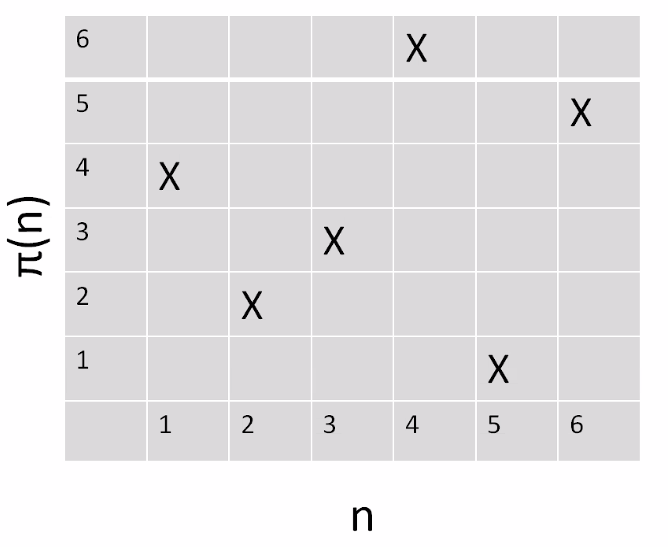
\includegraphics[scale=0.40]{img/main_permutation.PNG}
\end{center}
This graph represents the permutation \code{423615}:
\begin{itemize}
    \item $\pi(1) = 4$.
    \item $\pi(2) = 2$.
    \item $\pi(3) = 3$.
    \item $\pi(4) = 6$.
    \item $\pi(5) = 1$.
    \item $\pi(6) = 5$.
\end{itemize}
Suppose I selected three elements from the above graph (call this graph \code{1}):
\begin{center}
    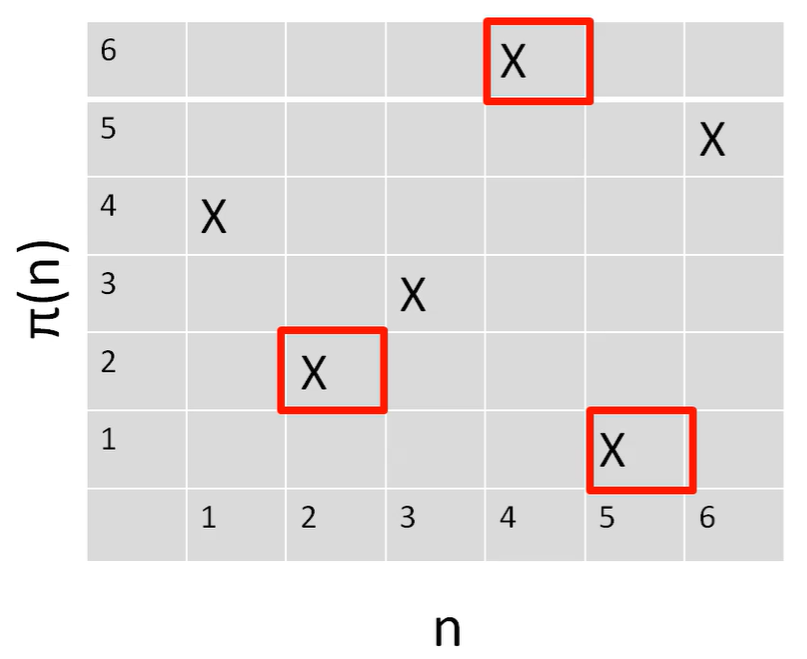
\includegraphics[scale=0.3]{img/main_permutation_s.PNG}
\end{center}
And now suppose that we have the following graph (call this graph \code{2}):
\begin{center}
    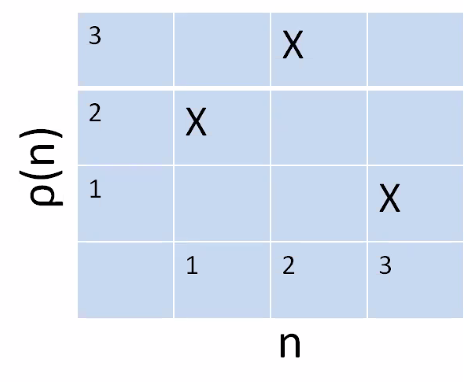
\includegraphics[scale=0.45]{img/pattern_perm.PNG}
\end{center}
Then, if we see the relative positions of the selected elements in graph \code{1}, we notice that they have the same relative positions as the three elements in graph \code{2}. In this sense, we can say that \code{261} has the same relative order as \code{231}, so \code{261} is a copy of the pattern \code{231} showing up within this larger permutation. 

\subsection{Pattern Avoidance}
\begin{definition}{}{}
    For a permutation $\rho$, let $S_{n}(\rho)$ be the set of permutations of $[n]$ that avoid $\rho$. 
\end{definition}
\textbf{Remark:} By avoid $\rho$, we mean the permutation that does not contain a copy of $\rho$. 

\subsubsection{Counting}
How many stack-sortable permutations are there? In other words, what is $|S_{n}(231)|$? 
\begin{theorem}{}{}
    \[|S_{n}(231)| = C_n\]
    Where $C_n$ is the $n$th Catalan Number.
\end{theorem}
\begin{proof}
    Let $A_{n} = |S_{n}(231)|$. We will show that $A_n$ satisfies the same recurrence as $C_n$. Namely:
    \begin{itemize}
        \item $A_0 = 1$ (Counting the empty permutation).
        \item $A_n = \sum_{k} A_{k - 1} A_{n - k}$. 
    \end{itemize}
    Consider $n$ in the $k$th location. We're going to assume that the biggest element $n$ shows up in the $k$th spot. That is:
    \begin{center}
        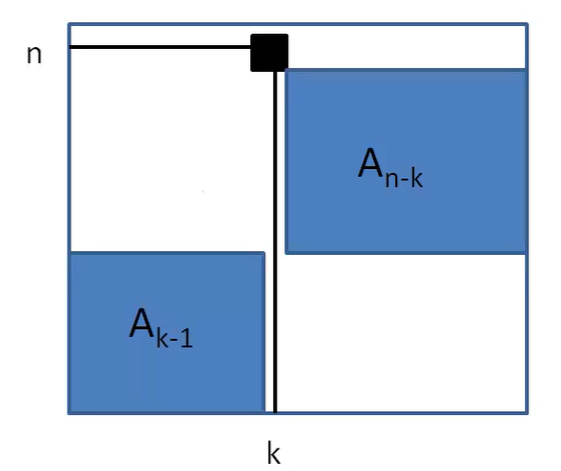
\includegraphics[scale=0.3]{img/layout_perm.PNG}
    \end{center}
    Because we don't have any copies of \code{231} (in particular, we don't have any copies where $n$ fills in this \code{3} position), the entries on the left must be smaller than entries on the right.
    \begin{itemize}
        \item The entries on the left are $1, 2, \dots, k - 1$.
        \item The entries on the right are $k + 1, \dots, n$. 
    \end{itemize} 
    The entries on the left and right must be 231-avoiding. So, the number of possibilities is $A_{k - 1}A_{n - k}$. Summing over $k$ gives the full value of $A_n = \sum_{k} A_{k - 1}A_{n - k}$. This shows the recursion holds and completes our proof.  
\end{proof}

\subsection{Rotations}
\begin{lemma}{}{}
    \[|S_{n}(231)| = |S_{n}(132)| = |S_{n}(312)| = |S_{n}(213)|\]
\end{lemma}
\begin{proof}
    Note that the diagrams for these permutations are simply rotations of each other.
    \begin{center}
        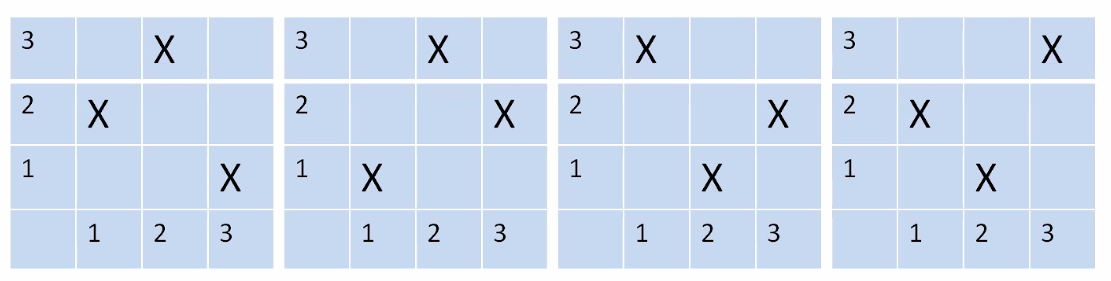
\includegraphics[scale=0.4]{img/perm_rotation.PNG}
    \end{center}
    For a permutation $\pi$, let $R\pi$ be its 90 degree permutation ($\pi$ contains a copy of $\rho$ if and only if $R\pi$ contains $R\rho$). Therefore, for any $\rho$, $|S_{n}(\rho)| = |S_{n}(R\rho)|$. The permutations that avoid $R\rho$ are just the rotations of those that avoid $\rho$, so there's a natural bijection. Then, applying this to $\rho = 231$ gives our theorem. 
\end{proof}

\subsection{Final Pattern}
Consider $|S_{n}(123)| = |S_{n}(321)|$. We make use of the theorem:
\begin{theorem}{}{}
    For all $n$, $|S_{123}| = |S_{n}(132)| = C_n$. 
\end{theorem} 
We want to show a bijection between the two. 

\subsubsection{Left-to-Right Minima}
We will use the following definition:
\begin{definition}{}{}
    The \textbf{left-to-right minima} of a permutation $\pi$ are all of the indices $i$ so that $\pi(i) < \pi(j)$ for all $j < i$. 
\end{definition}

An example of the left-to-right minima is:
\begin{center}
    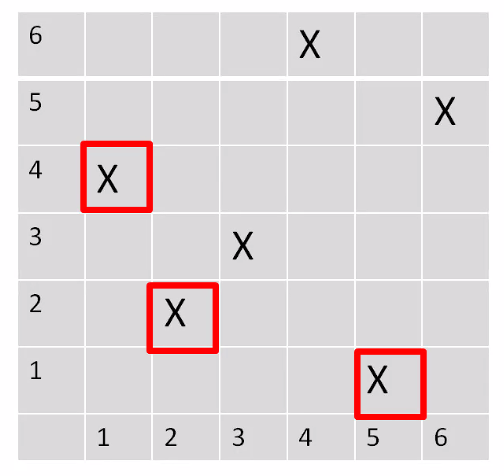
\includegraphics[scale=0.4]{img/selected_perm.PNG}
\end{center}

\subsubsection{Validity}
We want to classify permutations based on the locations (in the permutation graph) of their left-to-right minima.
\begin{definition}{}{}
    A set of pairs $(i, j)$ with $1 \leq i$ and $j \leq n$ is valid is:
    \begin{enumerate}
        \item They can be ordered $(i_1, j_1)$, $(i_2, j_2)$, \dots, $(i_k, j_k)$ so that $i_1 < i_2 < \dots < i_k$ and $j_1 > j_2 > \dots > j_k$.\footnote{They have to be decreasing.}
        \item For each $1 \leq a \leq n$, if $i_{\text{last}}$ is the largest of the $i$s less than or equal to $a$, then $j_{\text{last}} \leq n + 1 - a$.
    \end{enumerate}
\end{definition}

\begin{lemma}{}{}
    A set of pairs can be the set of left-to-right minima of a permutation of $[n]$ only if it is valid. 
\end{lemma}

\subsubsection{Minima to Permutations}
\begin{proposition}
    For every valid set $S$ of pairs, there is exactly one $123$-avoiding permutation and exactly one $132$-avoiding permutation with $S$ as its set of left-to-right minima. 
\end{proposition}


\subsubsection{123-Avoiding}
\begin{lemma}{}{}
    The non-left-to-right minima in a 123-avoiding permutation are in decreasing order.
\end{lemma}

\begin{proof}
    Suppose that this isn't the case.
    \begin{itemize}
        \item You have $(i_1, j_1)$ and $(i_2, j_2)$ with $i_1 < i_2$ and $j_1 < j_2$. 
        \item Since $(i_1, j_1)$ is not a minimum, there is an $(i_0, j_0)$ with $i_0 < i_1$ and $j_0 < j_1$. 
        \item Then, $(i_0, j_0)$, $(i_1, j_1)$, and $(i_2, j_2)$ is a copy of 123. \qedhere
    \end{itemize}
\end{proof}

Therefore, for every valid set, there is exactly one 123-avoiding permutation with those left-to-right minimums. 
\begin{itemize}
    \item Only one since the other terms must come in decreasing order. 
    \item Condition (2) implies that none of these will be a new minimum. 
    \item Left-to-right minima decreasing, which means the others are decreasing and threfore, we cannot have a three term increase.
\end{itemize}

\subsubsection{132-Avoiding}
We will construct our 132-avoiding permutation from the left-to-right minima set one step at a time.
\begin{itemize}
    \item We note that $\pi(1)$ will always be one of the left-to-right minima. 
    \item If $\pi(2)$ is not a left-to-right minima, we define it. 
    \item If $\pi(3)$ is not a left-to-right minima, we define it.
\end{itemize}

\subsubsection{Values}
\begin{lemma}{}{}
    When producing a 132-avoiding permutation, each new value must be the smallest not-yet-used value that is larger than the previous left-to-right minimum.
\end{lemma}

\begin{proof}
    We know that this:
    \begin{itemize}
        \item Cannot be smaller than previous left-to-right minimum. Otherwise it would be a left-to-right minimum
        \item Cannot be previously used value (this is a permutation). 
        \item Cannot be a non-minimum value. Otherwise it, the minimum value (whenever it shows up), and the previous left-to-right minimum will be a 132 pattern. \qedhere
    \end{itemize}
\end{proof}

\subsection{Pattern Comparison}
\begin{theorem}{}{}
    \[|S_{n}(1234) \leq |S_{n}(1324)|\]
\end{theorem}
We are going to count the number of permutations with a fixed set of left-to-right minima and a fixed set of right-to-left maxima. 

\subsubsection{1234-Avoiding}
\begin{lemma}{}{}
    For a 1234-avoiding permutation, the ``everything else'' (not a minima or maxima) must be sorted in decreasing order.
\end{lemma}

\subsubsection{1324-Avoiding}
\begin{lemma}{}{}
    For every set of left-to-right minima and right-to-left maxima that admits some permutation, there is at least one consistent 1324-avoiding permutation. 
\end{lemma}

\subsubsection{Idea}
The way we can construct this is through a swapping operation. 
\begin{itemize}
    \item If there is a \code{1324} in the permutation, take the \code{3} and \code{2} and swap them. 
    \item If you keep doing this, eventually there will be a point where there won't be anymore \code{1324}s in the permutation. 
    \item As a result, you will have a permutation that is \code{1324}-avoiding.
\end{itemize}

\subsubsection{Proof of Result}
\begin{itemize}
    \item Each sequence of left-to-right minima and right-to-left maxima that admits a permutation has at most 1 corresponding 1234-avoiding permutation and at least 1 corresponds 1324-avoiding permutation.
\end{itemize}
Therefore:
\[|S_{n}(1234)| \leq \#\{\text{Min/Max Patterns}\} \leq |S_{n}(1324)|\]

\textbf{Remark:} For $n \geq 7$, the inequality is strict. We need to show that two 1324-avoiding permuations with the same min/max sequence. 

\subsection{Asymptotics}
For every permutation $\rho$, there exists a constant $C$ so that for all $n$:
\[|S_{n}(\rho) \leq (C_{\rho})^n\]

\subsubsection{Asymptotic Result}
What if we take $\rho = 123\dots k$?

\begin{theorem}{}{}
    \[|S_{n}(123\dots k)| \leq (k - 1)^{2n}\]
\end{theorem}

\begin{proof}
    Split points into levels. 
    \begin{itemize}
        \item The first level is the left-to-right minima. 
        \item The $k$th level is the left-to-right minima after removing the first $(k - 1)$th level. \qedhere
    \end{itemize}
\end{proof}

So, a permutation that avoids $123\dots k$ has at most $k - 1$ levels and the points in each level are sorted. 

\subsubsection{Erdos-Szekeres}
The only way to avoid $123\dots k$ is to have few levels. These levels must be decreasing. 

\begin{theorem}{}{}
    Any permutation of $(n - 1)(m - 1) + 1$ contains a copy of $123\dots n$ or a copy of $m\dots 321$. 
\end{theorem}

\begin{proof}
    If you have $n$ or more levels, then you have $123\dots n$. Otherwise, pigeonhole implies a level with $m$, which gives a copy of $m\dots 321$. 
\end{proof}

\subsubsection{Permutation Sums}
\begin{definition}{}{}
    Given two permutations, $p$ and $q$, define their sum $p \oplus q$ to be the permutation whose graphs are given as follows:
    \begin{center}
        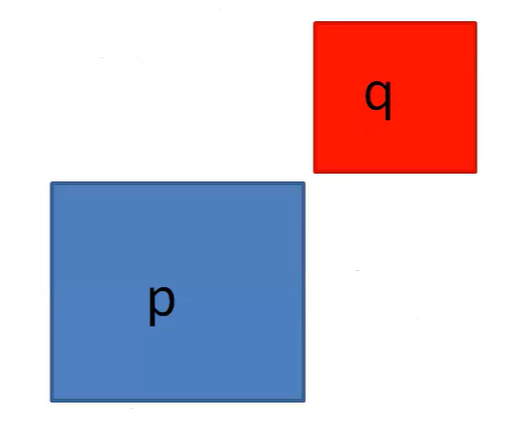
\includegraphics[scale=0.5]{img/p_sum.PNG}
    \end{center}
\end{definition}

\subsubsection{Sum Exponential Growth}
\begin{theorem}{}{}
    Let $p$ and $q$ be permutations with:
    \[|S_{n}(p \oplus 1)| \leq C_{p}^n\]
    \[|S_{n}(1 \oplus q)| \leq C_{q}^n\]
    Then:
    \[S_{n}(p \oplus 1 \oplus q)| \leq (\sqrt{C_p} + \sqrt{C_q})^{2n}\]
\end{theorem}







% --------------------------------------------------------- %
%                   NEW SECTION                             %
% --------------------------------------------------------- %
\newpage 
\section{Partial Orders}
\begin{itemize}
    \item Basic Definitions. 
    \item Dillworth's Theorem
    \item Incidence Algebras and Mobius Inversions. 
\end{itemize}

\subsection{Partial Orders}
\begin{definition}{}{}
    A \textbf{partial order} is a relation $\geq$ on a set satisfying three properties. 
    \begin{itemize}
        \item $x \geq x$ for all $x$ (reflexivity). 
        \item If $x \geq y$ and $y \geq z$, then $x \geq z$ (transitivity). 
        \item If $x \geq y$ and $y \geq x$, then $x = y$. 
    \end{itemize}
\end{definition}

\textbf{Remark:} There may be an $x$ and $y$ that are \underline{incomparable} (i.e. where neither $x \geq y$ nor $y \geq x$). In this sense, when we say \textbf{partial} order, we get some partial information (e.g. some things are bigger and so on). 


\subsection{Finite Partial Orders}
We will study some of the combinatorics of finite partial orders on finite sets. 

\subsubsection{Subsets}
$B_n$ is the collection of \textbf{subsets} of $[n]$ ordered by inclusion. 
\begin{itemize}
    \item $A \geq B$ if and only if $A \supseteq B$ ($A$ contains $B$)
    \item $2^n$ total elements. 
\end{itemize}

\subsubsection{Set Partitions and Refinements}
$\sqcap_n$ is the set of set partitions of $[n]$ ordered by \textbf{refinement}. 

\bigskip 

What is a refinement? A partition $P$ is $\geq$ a partition $Q$ if and only if $Q$ can be obtained from $P$ by breaking up the parts of $P$ into smaller parts. For example:
\begin{itemize}
    \item $\{1, 3, 4\}\{2, 5, 6\} \geq \{1\} \{3, 4\}\{2, 5, 6\}$ (We can obtain the latter partitions from the former by taking the element \code{1} out of its set in the former and putting it into its own set in the latter). 
\end{itemize}

\subsubsection{Natural Numbers and Divisiblity}
The natural numbers ($\N$) ordered by divisiblity. Specifically, $a \geq b$ if and only if $a$ is a multiple of $b$.

\bigskip 

For example, in this partial order:
\begin{itemize}
    \item $10 \geq 5$ is true because $10 = 5 \cdot 2$. 
    \item $10 \geq 7$ is false because 10 is not a multiple of 7.
\end{itemize}

\subsubsection{Real Numbers and Domination}
$\R^n$ ordered by domination. Namely, $(x_1, x_2, \dots, x_n) \geq (y_1, y_2, \dots, y_n)$ if and only if $x_1 \geq y_1$, $x_2 \geq y_2$, \dots, $x_n \geq y_n$. 

\subsubsection{Permutations and Patterns}
All permutations ordered by containment of patterns. Namely, $\pi \geq \rho$ if and only if $\pi$ contains a copy of $\rho$. 


\subsection{Min/Max}
\begin{definition}{}{}
    An element $x$ is in a partial order is:
    \begin{itemize}
        \item A \textbf{maximal} element if there is no $y > x$. 
        \item A \textbf{maximum} element if $x \geq y$ for all $y$. 
        \item A \textbf{minimal} element is there is no $y < x$. 
        \item A \textbf{minimum} element if $x \leq y$ for all $y$. 
    \end{itemize}
\end{definition}
Suppose we have a bunch of applicants for a job and these applicants are compared based on five different values. 
\begin{itemize}
    \item If there is a \textbf{maximum} element among these job applicants (someone that is better than everyone else in every values), then clearly that is the person you want to hire.
    \item If there isn't a maximum element, there might be several people where each of them are better than someone else at something. In this sense, you have a bunch of pairwise incomparable people. It's not clear \emph{who} you want among that group, but you probably want a \textbf{maximal} amount. You don't want to pick somebody where there was somebody else in your applicant pool that was just better than them in all categories that you care about. You at least want somebody that isn't strictly dominated by anyone else -- that would be a maximal element.
\end{itemize} 

\subsubsection{Example: Minimum Elements}
Which of the following have minimum elements? 
\begin{enumerate}[(a)]
    \item $B_n$
    \item $\sqcap_n$
    \item $\N$
    \item $\R^n$
\end{enumerate}

\begin{itemize}
    \item The answer is \code{A}, \code{B}, and \code{C}.
    \begin{itemize}
        \item For choice A ($B_n$), everything contains an empty set $\emptyset$. 
        \item For choice B ($\sqcap_n$), we can refine the elements so that every element in the set $[n]$ is in its own element. 
        \item For choice C ($\N$), we can have \code{1}, which is the minimum element possible that divides every other number. 
        \item For choice D ($\R^n$), we will always be able to find a smaller number. 
    \end{itemize}
\end{itemize}

\subsubsection{Example: Maximum Elements}
Which of the following have maximum elements? 
\begin{enumerate}[(a)]
    \item $B_n$
    \item $\sqcap_n$
    \item $\N$
    \item $\R^n$
\end{enumerate}

\begin{itemize}
    \item The answer is \code{A} and \code{B}.
    \begin{itemize}
        \item For choice A ($B_n$), the biggest element is $\{1, 2, 3, \dots, n\}$.
        \item For choice B ($\sqcap_n$), the biggest element is (again) $\{1, 2, 3, \dots, n\}$.
        \item For choices C and D ($\N$ and $\R^n$, respectively), we can keep finding bigger elements. 
    \end{itemize}
\end{itemize}


\subsection{Covering Elements}
\begin{definition}{}{}
    We say that $x$ \underline{covers} $y$ if $x > y$ but there is no $z$ with $x > z > y$. 
\end{definition}

\begin{lemma}{}{}
    In any finite partial order, $x \geq y$ if and only if there is some chain of elements $x = x_0, x_1, \dots, x_n = y$ with $x_i$ covering $x_{i + 1}$. 
\end{lemma}
This means that if we know which elements cover which other elements, we will be able to recover the partial order. 


\subsection{Hasse Diagram}
The lemma implies that you can specify the partial order by specifying which elements cover which others. 

\begin{definition}{}{}
    The \textbf{Hasse Diagram} of a partial order draws the elements of the partial order with lines between $x$ and $y$ if $x$ covers $y$, and with $x$ positioned vertically above $y$.
\end{definition}

\subsubsection{Example: Hasse Diagram for Refinement}
Consider the Hasse Diagram for $\sqcap_3$:
\begin{center}
    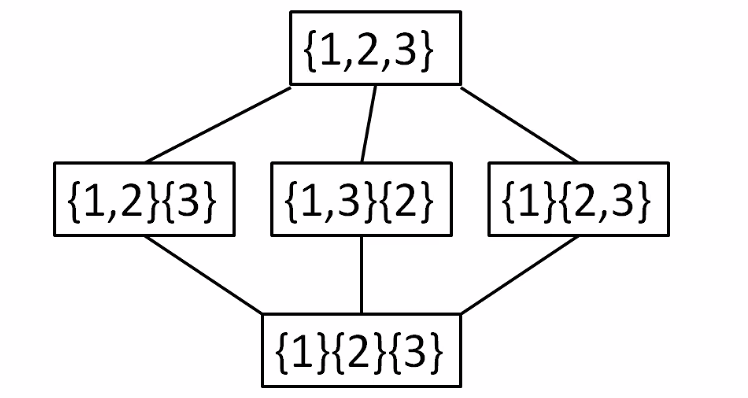
\includegraphics[scale=0.5]{img/ex_hasse.PNG}
\end{center}
Where the bottom-most element is the minimum element and the top-most element is the maximum element. 

\subsection{Chains and Anti-Chains}
\begin{definition}{}{}
    A \textbf{chain} in a partial order is a sequence of elements
    \[x_1 < x_2 < x_3 < \dots < x_k\]
\end{definition}

\begin{definition}{}{}
    An \textbf{anti-chain} in a partial order is a collection of elements $x_i$ so that no two of the $x_i$ are comparable. 
\end{definition}

\textbf{Remark:}
\begin{itemize}
    \item A chain is a big sequence of elements pairwise are comparable to each other. Every element in this chain can be compared to every other element in this chain. 
    \item An anti-chain is sort of the opposite. It's essentially a bunch of elements that are pairwise incomparable. 
\end{itemize}

\subsubsection{Covers by Chains}
\begin{definition}{}{}
    Given a partial order, a \textbf{cover} by chains is a collection of chains whose union is all of the elements of the order. 
\end{definition}

\subsubsection{Example: Covers of \texorpdfstring{$\sqcap_3$}{Set of Set Partitions of [3] Ordered by Refinement}}
What is the smallest number of chains needed to cover $\sqcap_3$?
\begin{center}
    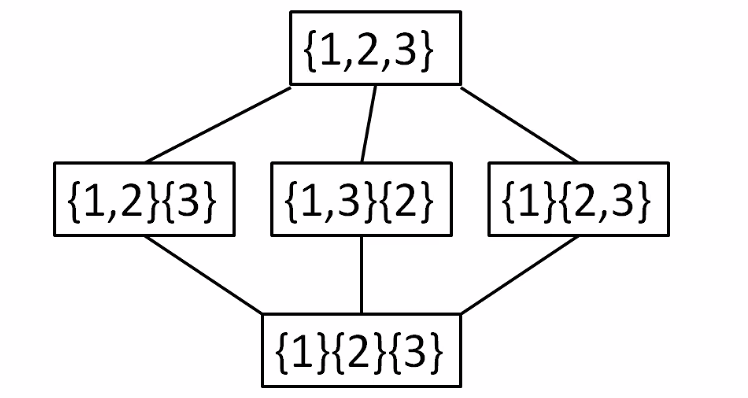
\includegraphics[scale=0.3]{img/ex_hasse.PNG}
\end{center}

\begin{itemize}
    \item There are \textbf{3} chains. They are shown below:
    \begin{itemize}
        \item $1|2|3 \to 12|3 \to 123$.
        \item $1|2|3 \to 13|2 \to 123$.
        \item $1|2|3 \to 1|23 \to 123$.
    \end{itemize}
    Diagrammatically, this looks like:
    \begin{center}
        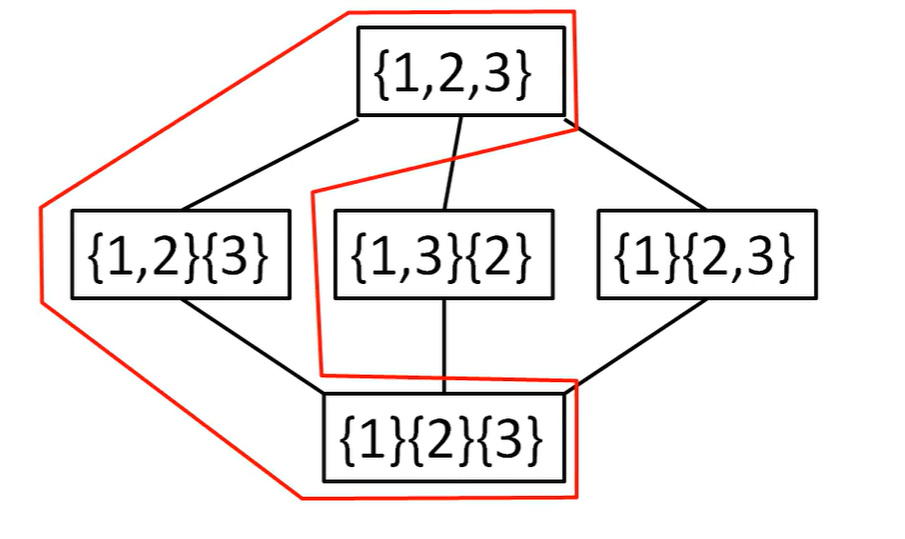
\includegraphics[scale=0.25]{img/hasse_1.PNG}
        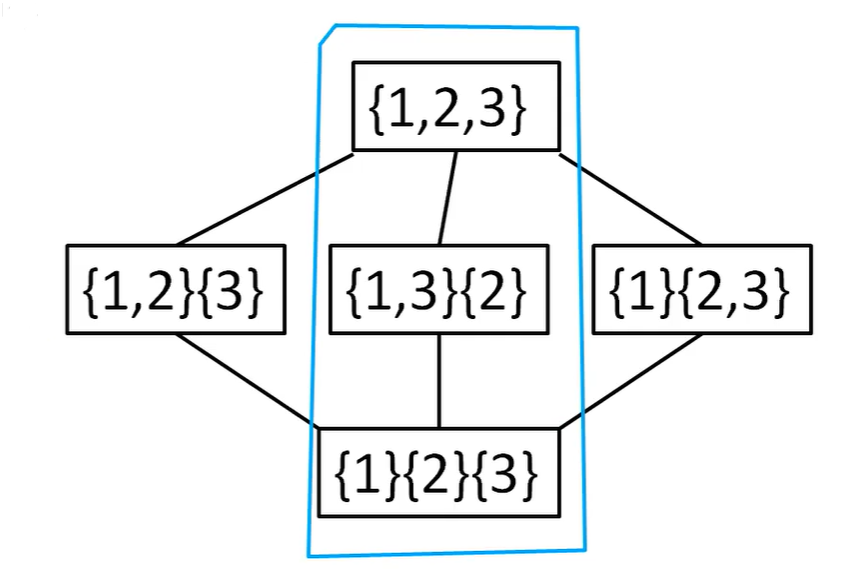
\includegraphics[scale=0.25]{img/hasse_2.PNG}
        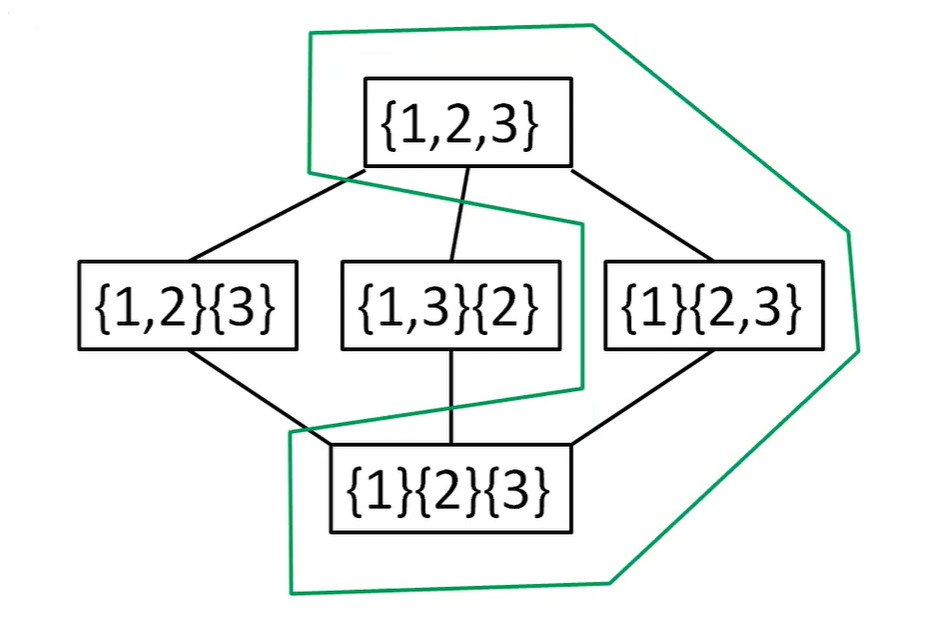
\includegraphics[scale=0.25]{img/hasse_3.PNG}
    \end{center}
    Combining these together gives:
    \begin{center}
        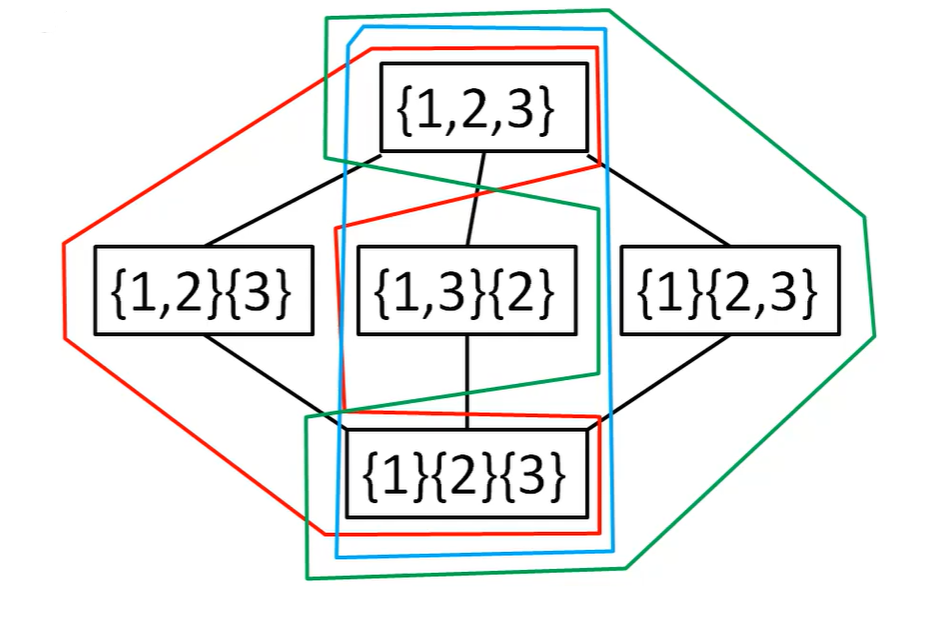
\includegraphics[scale=0.5]{img/hasse_4.PNG}
    \end{center}
\end{itemize}

\subsubsection{Dilworth's Theorem}
\begin{theorem}{Dilworth's Theorem}{}
    The size of any maximum antichain is equal to the number of chains in any smallest chain cover. 
\end{theorem}

With regards to the previous question, Dilworth's Theorem answers the question: \emph{How do we know we cannot use fewer than 3 chains? }
\begin{center}
    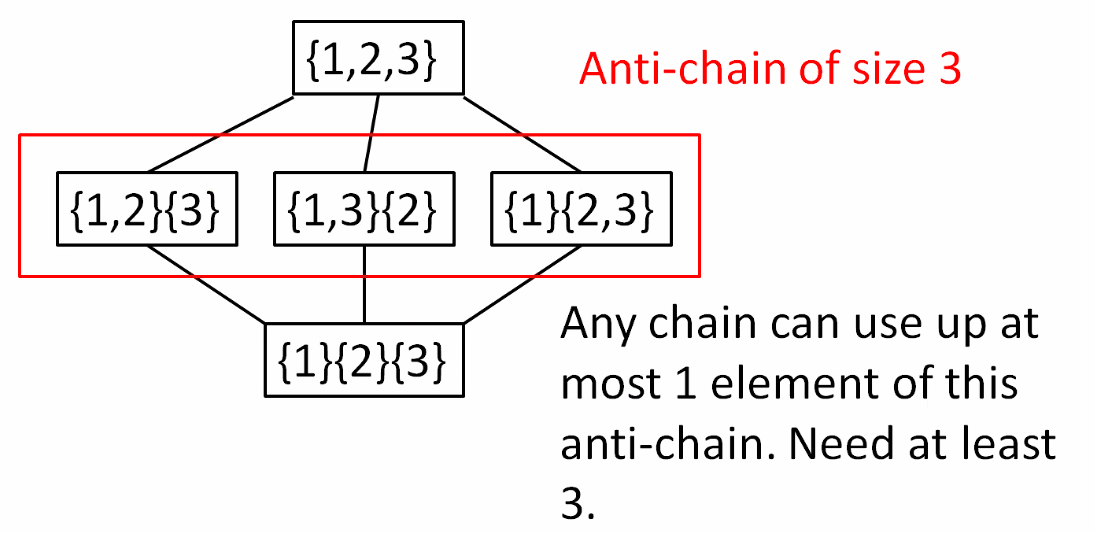
\includegraphics[scale=0.25]{img/hasse_dil.PNG}
\end{center}

The proof is a bit on the tedious side.
\begin{proof}
    We know that the minimum chain-cover is greater than or equal to maximum anti-chain. This is because if you have a chain covering an anti-chain, each chain in the cover can intersect at most one element in the anti-chain, and because they have to cover the whole anti-chain, the number of chains in the cover needs to be at least the number of points in the anti-chain. 
    
    \bigskip 

    Now, we need to prove by strong induction on the size of the partial order $P$. This is significantly more difficult.
    \begin{itemize}
        \item[\mdiamond] \underline{Base Case:} If $|P| = 1$, the size of the maximum chain is equal to 1, which is equal to the size of the minimum chain. 
        \item[\mdiamond] \underline{Inductive Step:} Suppose Dilworth's Theorem holds for all partial orders with fewer than $|P|$ elements. Let $A$ be an maximal anti-chain. Then, every other element $x$ in $P$ must be comparable to some element of $A$. Otherwise, $A \cup \{x\}$ would be a bigger anto-chain. 
        
        \bigskip 

        Each $x$ can be bigger than some element of $A$ or smaller, but not both. For example, if $x > a_1$ and $x < a_2$, then by transitivity we have $a_1 < x < a_2$, which means that these two elements are comparable and thus $A$ is not an anti-chain. 

        We can partition the elements of $P$ into 3 sets. 
        \begin{itemize}
            \item $A$ 
            \item $U$, the set of elements bigger than some element in $A$. 
            \item $L$, the set of elements less than some elements in $A$. 
        \end{itemize}
        This looks like:
        \begin{center}
            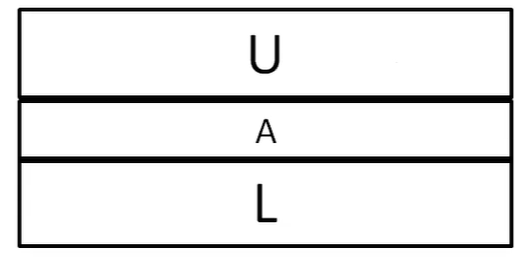
\includegraphics[scale=0.5]{img/dil_pic_proof.PNG}
        \end{center}

        Now, consider these cases.
        \begin{itemize}
            \item \underline{Case 1:} Suppose that there is some maximal anti-chain $A$ so that both $U$ and $L$ are non-empty. Then, applying the inductive hypothesis to $A \cup L$ and $A \cup U$, we know that $A$ is still a maximal anti-chain for each of these partial orders and, therefore, by the inductive hypothesis, there are chain covers of size $|A|$ for each chain. Now, the only way we can have chain covers of sizes exactly the size of $A$ is if each element in $A$ is in exactly one chain in each cover. So, gluing the upper and lower chain covers together:
            \begin{itemize}
                \item We can combine the chain from $A \cup U$ with $x \in A$ with the chain in $A \cup L$ with $x$ to get the new chain. 
                \item These chains cover $L \cup A \cup U = P$.
            \end{itemize}

            \item \underline{Case 2:} Suppose that every maximal anti-chain $A$ either has $L = \emptyset$ or $U = \emptyset$. Then, every maximal anti-chain either contains all minimal elements of $P$ or all maximal elements of $P$. Otherwise, a minimal element will be in $L$ and a maximal element will be in $U$. Then, suppose we find a maximal element $x$ and a minimal element $y$ with $x \geq y$. Then, every element is bigger than some minimal element. Additionally, from our assumptions, every maximal anti-chain contains either $x$ or $y$. This means that $P - \{x, y\}$ has a smaller maximum anti-chain. In particular, letting $k$ be the size of the maximum anti-chain of $P$. Then, $P - \{x, y\}$ has the maximum anti-chain of size at most $k - 1$. By the inductive hypothesis, we can cover $P - \{x, y\}$ with the chains $C_1, C_2, \dots, C_{k - 1}$. This can cover $P$ with chains $C_1, C_2, \dots, C_{k - 1}, \{x, y\}$. 
        \end{itemize}
        This completes our inductive proof.
    \end{itemize}
    Hence, this completes this proof. \qedhere
\end{proof}

\subsection{Incidence Algebra}
\begin{definition}{}{}
    For a partial order $P$, let\footnote{The set of all comparable things.}:
    \[\text{Int}(P) = \{(x, y) \mid x, y \in P, x \leq y\}\]
    Here, $\text{Int}$ means the interval. So, the above means the set of intervals of $P$. 
\end{definition}
The \textbf{incidence algebra} of $P$ is the set of functions:
\[f: \text{Int}(P) \to \R\]

\bigskip 

This has a multiplication operation:
\[(f \cdot g)(x, y) := \sum_{x \leq w \leq y} f(x, w)g(w, y)\]

\textbf{Remark.} Similar to recursion for $f_m$. 

\subsubsection{Identity}
The incidence algebra has an identity:
\[\delta(x, y) = \begin{cases}
    1 & x = y \\ 
    0 & \text{Otherwise}
\end{cases}\]
Essentially:
\[(f \cdot \delta)(x, y) = \sum_{x \leq w \leq y} f(x, w)\delta(w, y) = f(x, y)\]
\textbf{Remark.} The only non-zero term in the sum is when $w = y$. 

\subsubsection{Zeta}
Another useful member of the incidence algebra is the following:
\[\zeta(x, y) = 1 \qquad \forall x \leq y\]

\textbf{Claim.} The number of chains of length $k$ from $x$ to $y$ is:
\[\underbrace{(\zeta - \delta) \cdot (\zeta - \delta) \cdot \dots (\zeta - \delta)(x, y)}_{k - 2 \text{ Times}}\]

\begin{proof}
    Let $D = \zeta - \delta$. Then:
    \[D(x, y) = \begin{cases}
        1 & x < y \\
        0 & \text{Otherwise}
    \end{cases}\]
    Then:
    \begin{equation*}
        \begin{aligned}
            (D \cdot D \cdot \dots \cdot D)(x, y) &= \sum_{x \leq w_1 \leq w_2 \leq \dots \leq w_{k - 2} \leq y} D(x, w_1)D(w_1, w_2) \dots D(w_{k - 3}, w_{k - 2})D(w_{k - 2}, y) \\ 
                &= \sum_{x < w_1 < w_2 < \dots < w_{k - 2} < y} 1 \\ 
                &= \text{Number of length } k \text{ chains from } x \text{ to } y
        \end{aligned}
    \end{equation*}
\end{proof}

\subsubsection{Inverses}
We have that $\delta$ acts as an identity element for the incidence algebra. What about inverses? 

\begin{lemma}{}{}
    For any function $f$ with $f(x, x)$ being non-zero for all $x$ in $P$, there is a $g$ so that $(f \cdot g) = \delta$. 
\end{lemma}

\subsection{Mobius Function}
Of particular interests is the inverse of $\zeta$, commonly denoted by $\mu$.

\bigskip 

For $\mu(x, x) = 1$ and for $x < y$, we have:
\[0 = \sum_{x \leq w \leq y} \zeta(x, w) \mu(w, y) = \sum_{x \leq w \leq y} \mu(w, y)\]
In particular:
\[\mu(x, y) = -\sum_{x \leq w < y} \mu(w, y)\]

\subsubsection{Example 1: \texorpdfstring{$B_n$}{B}}
For two sets $S \subseteq T$, we have:
\[\mu(S, T) = (-1)^{|T| - |S|}\]
To verify that this works, suppose that $|T| - |S| = k > 0$. There are $\binom{k}{m}$ subsets $S \subseteq R \subseteq T$ with $|T| - |R| = m$ (we take a subset of $T - S$ of size $m$). Thus:
\[\sum_{S \subseteq R \subseteq T} \mu(R, T) = \sum_{m = 0}^{k} \binom{k}{m} (-1)^m = 0\]

\subsubsection{Example 2: \texorpdfstring{$\N$}{Natural Numbers}}
To compute $\mu(n, m)$, write $\frac{m}{n}$ as a product of primes $p_1 p_2 \dots p_k$. Then:
\[\mu(n, m) = \begin{cases}
    (-1)^k & \pi \text{ are distinct} \\ 
    0 & \text{Otherwise}
\end{cases}\]
To show that this works, we need to show that the sum of $\mu(d, m)$ over all $n | d | m$ is 0. We note that if $\frac{m}{n}$ is divisible by $k$ distinct primes, there will be $\binom{k}{t}$ such $d$s where $\frac{m}{d}$ is a product of $t$ distinct primes (choose which primes from the $k$). The computation, then, is similar to the previous example. 

\subsubsection{Example 3: Partial Order}
An example can be found at the end. 

\subsection{Mobius Inversion}
\begin{theorem}{}{}
    Given two functions $f$ and $g$ on $P$ with:
    \[g(x) = \sum_{x \leq y} f(y)\]
    We have that:
    \[f(y) = \sum_{y \leq x} g(x) \mu(y, x)\]
\end{theorem}

\subsection{Products of Partial Orders}
\begin{definition}{}{}
    If $P$ and $Q$ are partial orders, the product partial order is defined in the set $P \times Q$ where $(x_1, x_2)$ is $\leq (y_1, y_2)$ if and only if $x_1 \leq y_1$ and $x_2 \leq y_2$. 
\end{definition}

\subsubsection{Example: \texorpdfstring{$\R$ and $B_n$}{R and B}}
\[\R^n = \underbrace{\R^1 \times \R^1 \times \dots \times \R^1}_{n \text{ Times}}\]
\[B_n = \underbrace{B_1 \times B_1 \times \dots \times B_1}_{n \text{ Times}}\]
Each copy of $B_1$ asks if a single element is in the set. 
\[\N \text{ is a product over primes.}\]
For each $p$, we have a partial order on $\{1, p, p^2, p^3, \dots\}$. $\N$ is equivalent to the partial order on the product of these. 

\subsubsection{Mobius on Products}
\begin{theorem}{}{}
    We have for partial orders $P$ and $Q$:
    \[\mu_{P \times Q}((x, x'), (y, y')) = \mu_{P}(x, y) \mu_{Q}(x', y')\]
\end{theorem}

\begin{proof}
    It is enough to show that this satisifies the definition. 
    \[\sum_{(x, x') \leq (w, w') \leq (y, y')} \mu_{P}(w, y) \mu_{Q}(w', y') = \left(\sum_{x \leq w \leq y} \mu_{P}(w, y)\right)\left(\sum_{x' \leq w' \leq y'} \mu_{Q}(w', y')\right) = \delta((x, x'), (y, y'))\]
\end{proof}

\subsection{Lattices}
Another special case:
\begin{definition}{}{}
    A partial order is a lattice if for every two elements $x$, $y$ we have:
    \begin{itemize}
        \item A minimum upper bound: $a = x \vee y$
        \item A maximum lower bound: $b = x \wedge y$.
    \end{itemize}
    In particular:
    \begin{itemize}
        \item $z \geq x$ and $z \geq y$ if and only if $z \geq a$. 
        \item $z \leq x$ and $z \leq y$ if and only if $z \leq b$. 
    \end{itemize}
\end{definition}

From the book:
\begin{definition}{}{}
    A partial order is called a lattice if any two elements $x$ and $y$ of said partial order have a minimum common upper bound $a$, and a maximum common lower bound $b$. 
    
    \bigskip 
    
    Here, $a$ is called the \emph{join} of $x$ and $y$, and $b$ is called the \emph{meet} of $x$ and $y$. We denote these relations by $x \vee y = a$ and $x \wedge y = b$. 
\end{definition}

\subsubsection{Example: Lattices}
\emph{Which of the following partial orders are lattices?}
\begin{enumerate}[(a)]
    \item $B_n$
    \item $\N$
    \item $\R^n$
\end{enumerate}

\begin{itemize}
    \item The answer is all of them. 
    \begin{itemize}
        \item $B_n$: Union/intersection. 
        \item $\N$: LCM/GCD. 
        \item $\R^n$: Coordinate-wise max/min. 
    \end{itemize}
\end{itemize}

\subsubsection{Minimums and Maximums}
\begin{lemma}{}{}
    Any finite lattice has minimum and maximum elements. 
\end{lemma}

\begin{proof}
    Take the minimum upper bound and maximum lower bound of all elements.
\end{proof}

\subsubsection{Another Criteria}
\begin{lemma}{}{}
    If a finite partial order $P$ has a maximum element and has maximum lower bounds, it is a lattice. 
\end{lemma}

\begin{proof}
    Need to show that for any $x$ and $y$, we have a minimum upper bound. Take the maximum lower bound of all upper bounds of $x$ and $y$ (exist because maximum). 
\end{proof}

\subsubsection{An Application: Refinement}
\begin{corollary}{}{}
    $\sqcap_n$ is a lattice.    
\end{corollary}

\begin{proof}
    $\sqcap_n$ is finite, has a maximum element ($[n]$), and has maximum lower bounds (common refinement). 
\end{proof}


\subsection{Weisner's Theorem}
\begin{theorem}{}{}
    Let $P$ be a lattice with maximum element 1 and minimum element 0. Then, for any $a \neq 1$:
    \[\mu(0, 1) = -\sum_{\substack{x \wedge a = 0 \\ x \neq 0}} \mu(x, 1)\]
\end{theorem}

\begin{proof}
    We need to show that:
    \[\sum_{x: x \wedge a = 0} \mu(x, 1) = 0\]
    Define the function $f$ on $P$ by:
    \[f(x) := \begin{cases}
        1 & x \wedge a = 0 \\ 
        0 & \text{Otherwise}
    \end{cases} = \sum_{\substack{y \leq a \\ y \leq x}} \mu(0, y)\]
    We have that:
    \[\sum_{x: x \wedge a = 0} \mu(x, 1) = \sum_x \mu(x, 1)f(x) = \sum_x \sum_{\substack{y \leq x \\ y \leq a}} \mu(x, 1) \mu(0, y) = \sum_{y \leq a} \mu(0, y) \underbrace{\sum_{x \geq y} \mu(x, 1)}_{\text{Always } 0} = 0\]
\end{proof}

\subsection{Practice Problem}
Here are some random practice problems. 

\subsubsection{Example: Hasse Diagram}
Consider the following Hasse Diagram\footnote{Thanks to TA Jesse Kim for this drawing.}:
\begin{center}
    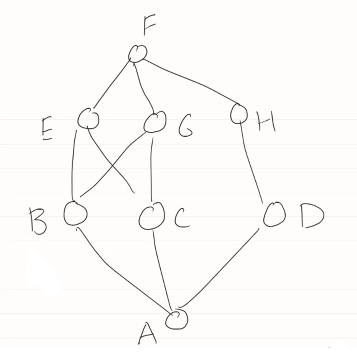
\includegraphics[scale=0.6]{img/mobius.PNG}
\end{center}
\begin{itemize}
    \item Is this a lattice? 
    \item Find $\mu(A, F)$. 
    \item What is the largest anti-chain? What is the minimal chain cover? 
\end{itemize}

The solutions are as follows:
\begin{itemize}
    \item Let's begin by considering two cases. 
    \begin{itemize}
        \item Let's consider the two elements $B$ and $C$. Recall that an upper-bound for two elements $x$ and $y$ is an element $u$ such that $x \leq u$ and $y \leq u$. 
        \begin{itemize}
            \item First, what elements are above $B$? We have elements $G$, $E$, and $F$.  
            \item Now, what elements are above $C$? We have elements $E$, $G$, and $F$. 
        \end{itemize}
        Further, recall that two elements $x$ and $y$ have a minimum common upper-bound if there is \textbf{one} element $u$ that is the ``closet'' to both $x$ and $y$ such that $x \leq u$ and $y \leq u$. While it is true that both $B$ and $C$ share the same upper-bounds, $B$ and $C$ do \textbf{not} have a minimum common upper-bound (because there are two different ``minimum'' upper-bounds).  

        \item Let's now consider the two elements $E$ and $G$. Recall that a lower-bound for two elements $x$ and $y$ is an element $u$ such that $u \leq x$ and $u \leq y$. 
        \begin{itemize}
            \item First, what elements are below $E$? We have elements $B$, $C$, and $A$. 
            \item Now, what elements are below $G$? We have elements $B$, $C$, and $A$.  
        \end{itemize}
        By similar reasoning, while both $E$ and $G$ share the same lower-bounds, $E$ and $G$ do \textbf{not} have a maximum common lower-bound (because there are two different ``maximum'' lower-bounds). 
    \end{itemize}
    By this, it follows that the above Hasse Diagram does not represent a lattice. 
    
    
    % $E$ and $G$ do not share a maximum common lower-bound (the maximum lower-bound of $E$ is $C$ whereas the maximum lower-bound of $G$ is $B$). For similar reasons, the elements $B$ and $C$ do not share a minimum common upper-bound (the minimum upper-bound of $B$ is $G$ whereas the minimum upper-bound of $C$ is $E$). Thus, this is \emph{not} a lattice. 

    \item We know that:
    \[\mu(A, F) = -\sum_{A \leq Z < F} \mu(A, Z)\]
    We know that (this is given):
    \[\mu(A, A) = 1\]
    Consider the elements that connect directly to $A$. This is simply: 
    \[\mu(A, B) = \mu(A, C) = \mu(A, D) = -\mu(A, A) = -1\]
    Now, we know that:
    \[\mu(A, H) = -(\mu(A, A) + \mu(A, D)) = -(1 - 1) = 0\]
    \[\mu(A, E) = -(\mu(A, A) + \mu(A, B) + \mu(A, C)) = -(1 + -1 + -1) = 1\]
    \[\mu(A, G) = -(\mu(A, A) + \mu(A, B) + \mu(A, C)) = -(1 - 1 - 1) = 1\]
    \begin{equation*}
        \begin{aligned}
            \mu(A, F) &= -(\mu(A, A) + \mu(A, B) + \mu(A, C) + \mu(A, D) + \mu(A, E) + \mu(A, G) + \mu(A, H)) \\ 
                &= -(1 + (-1) + (-1) + (-1) + 1 + 1 + 0) \\ 
                &= -(3 - 3) \\ 
                &= 0
        \end{aligned}
    \end{equation*}
    \item \code{BCD}, \code{EGH}, \code{BCH}, and \code{EGD} are the largest anti-chains. By Dilworth's Theorem, the size of the largest anti-chain is 3, so there are 3 chains in the smallest chain cover. In this case, the 3 chains are \code{ABEF}, \code{ACGF}, and \code{ADHF}. 
\end{itemize}







% --------------------------------------------------------- %
%                   NEW SECTION                             %
% --------------------------------------------------------- %
\newpage 
\section{Appendix}
Here are some more information that may be helpful.

\subsection{Corresponding Lectures}
The following are the corresponding lectures. These may be useful if the notes don't cover everything. If you click on a link, make sure to right-click and open in a new tab. 

\begin{center}
    \begin{tabular}{|c|c|c|c|}
        \hline 
        \textbf{L} & \textbf{Topic} & \textbf{Video} & \textbf{Slides} \\ 
        \hline 
        1 & Weak Induction & \href{http://cseweb.ucsd.edu/~dakane/Math184/Lec1.html}{Link} & \href{http://cseweb.ucsd.edu/~dakane/Math184/Lec1.pdf}{Link} \\ 
        \hline
        2 & Strong Induction, Pigeonhole & \href{http://cseweb.ucsd.edu/~dakane/Math184/Lec2.html}{Link} & \href{http://cseweb.ucsd.edu/~dakane/Math184/Lec2.pdf}{Link} \\ 
        \hline
        3 & Generalized Pigeonhole, Basic Counting Techniques & \href{http://cseweb.ucsd.edu/~dakane/Math184/Lec3.html}{Link} & \href{http://cseweb.ucsd.edu/~dakane/Math184/Lec3.pdf}{Link} \\ 
        \hline
        4 & Multinomial Coefficients, Balls and Bins & \href{http://cseweb.ucsd.edu/~dakane/Math184/Lec4.html}{Link} & \href{http://cseweb.ucsd.edu/~dakane/Math184/Lec4.pdf}{Link} \\ 
        \hline
        5 & Stars and Bars, Set Partitions, Stirling Numbers & \href{http://cseweb.ucsd.edu/~dakane/Math184/Lec5.html}{Link} & \href{http://cseweb.ucsd.edu/~dakane/Math184/Lec5.pdf}{Link} \\ 
        \hline
        6 & Stirling Numbers, Bell Numbers, Integer Partitions & \href{http://cseweb.ucsd.edu/~dakane/Math184/Lec6.html}{Link} & \href{http://cseweb.ucsd.edu/~dakane/Math184/Lec6.pdf}{Link} \\ 
        \hline
        7 & Integer Partitions & \href{http://cseweb.ucsd.edu/~dakane/Math184/Lec7.html}{Link} & \href{http://cseweb.ucsd.edu/~dakane/Math184/Lec7.pdf}{Link} \\ 
        \hline
        8 & Permutations, Cycle Structures, Counting & \href{http://cseweb.ucsd.edu/~dakane/Math184/Lec8.html}{Link} & \href{http://cseweb.ucsd.edu/~dakane/Math184/Lec8.pdf}{Link} \\ 
        \hline
        9 & Counting Permutations, Stirling, Cycles w/ Specific Elements, Odd/Even & \href{http://cseweb.ucsd.edu/~dakane/Math184/Lec9.html}{Link} & \href{http://cseweb.ucsd.edu/~dakane/Math184/Lec9.pdf}{Link} \\ 
        \hline
        10 & Sizes of Cycles w/ Individual Elements, Odd/Even Cycles & \href{http://cseweb.ucsd.edu/~dakane/Math184/Lec10.html}{Link} & \href{http://cseweb.ucsd.edu/~dakane/Math184/Lec10.pdf}{Link} \\ 
        \hline
        11 & Computation of Even/Odd Cycles, Inclusion-Exclusion & \href{http://cseweb.ucsd.edu/~dakane/Math184/Lec11.html}{Link} & \href{http://cseweb.ucsd.edu/~dakane/Math184/Lec11.pdf}{Link} \\ 
        \hline
        12 & Inclusion-Exclusion, Applications & \href{http://cseweb.ucsd.edu/~dakane/Math184/Lec12.html}{Link} & \href{http://cseweb.ucsd.edu/~dakane/Math184/Lec12.pdf}{Link} \\ 
        \hline
        13 & Derangements, Binomial Theorem & \href{http://cseweb.ucsd.edu/~dakane/Math184/Lec13.html}{Link} & \href{http://cseweb.ucsd.edu/~dakane/Math184/Lec13.pdf}{Link} \\ 
        \hline
        14 & Generalizations of Binomial Theorem, Generating Functions & \href{http://cseweb.ucsd.edu/~dakane/Math184/Lec14.html}{Link} & \href{http://cseweb.ucsd.edu/~dakane/Math184/Lec14.pdf}{Link} \\ 
        \hline
        15 & Solving Recurrence Relations, Products of Generating Functions & \href{http://cseweb.ucsd.edu/~dakane/Math184/Lec15.html}{Link} & \href{http://cseweb.ucsd.edu/~dakane/Math184/Lec15.pdf}{Link} \\ 
        \hline
        16 & Applications of Generating Functions, Catalan Numbers & \href{http://cseweb.ucsd.edu/~dakane/Math184/Lec16.html}{Link} & \href{http://cseweb.ucsd.edu/~dakane/Math184/Lec16.pdf}{Link} \\ 
        \hline
        17 & Composition of Generating Functions & \href{http://cseweb.ucsd.edu/~dakane/Math184/Lec17.html}{Link} & \href{http://cseweb.ucsd.edu/~dakane/Math184/Lec17.pdf}{Link} \\ 
        \hline
        18 & Basics of Exponential Generating Functions & \href{http://cseweb.ucsd.edu/~dakane/Math184/Lec18.html}{Link} & \href{http://cseweb.ucsd.edu/~dakane/Math184/Lec18.pdf}{Link} \\ 
        \hline
        19 & Compositions of Generating Functions & \href{http://cseweb.ucsd.edu/~dakane/Math184/Lec19.html}{Link} & \href{http://cseweb.ucsd.edu/~dakane/Math184/Lec19.pdf}{Link} \\ 
        \hline
        20 & Applications of Compositions of EGF & \href{http://cseweb.ucsd.edu/~dakane/Math184/Lec20.html}{Link} & \href{http://cseweb.ucsd.edu/~dakane/Math184/Lec20.pdf}{Link} \\ 
        \hline
        21 & Patterns and Pattern Avoidance in Permutation & \href{http://cseweb.ucsd.edu/~dakane/Math184/Lec21.html}{Link} & \href{http://cseweb.ucsd.edu/~dakane/Math184/Lec21.pdf}{Link} \\ 
        \hline
        22 & Computing $|S_{n}(123)|$, Left-to-Right Minima & \href{http://cseweb.ucsd.edu/~dakane/Math184/Lec22.html}{Link} & \href{http://cseweb.ucsd.edu/~dakane/Math184/Lec22.pdf}{Link} \\ 
        \hline
        23 & Pattern Avoidance Asymptotics & \href{http://cseweb.ucsd.edu/~dakane/Math184/Lec23.html}{Link} & \href{http://cseweb.ucsd.edu/~dakane/Math184/Lec23.pdf}{Link} \\
        \hline 
        24 & Partial Orders, Chains, Examples & \href{http://cseweb.ucsd.edu/~dakane/Math184/Lec24.html}{Link} & \href{http://cseweb.ucsd.edu/~dakane/Math184/Lec24.pdf}{Link} \\ 
        \hline
        25 & Incidence Algebras, Inverses & \href{http://cseweb.ucsd.edu/~dakane/Math184/Lec25.html}{Link} & \href{http://cseweb.ucsd.edu/~dakane/Math184/Lec25.pdf}{Link} \\
        \hline 
        26 & Computing $\mu$ & \href{http://cseweb.ucsd.edu/~dakane/Math184/Lec26.html}{Link} & \href{http://cseweb.ucsd.edu/~dakane/Math184/Lec26.pdf}{Link} \\ 
        \hline
        27 & Professor Kane's Research & \href{http://cseweb.ucsd.edu/~dakane/Math184/Lec27.html}{Link} & \href{http://cseweb.ucsd.edu/~dakane/Math184/Lec27.pdf}{Link} \\ 
        \hline 
    \end{tabular}
\end{center}

\subsection{Common Generating Functions}
\begin{itemize}
    \item For the sequence of numbers: $1, 1, 1, 1, 1, \dots$
    \[x^0 + x^1 + x^2 + x^3 + x^4 + x^5 + \dots = \sum_{n = 0}^{\infty} x^n = \frac{1}{1 - x}\]
    \[\frac{x^0}{0!} + \frac{x^1}{1!} + \frac{x^2}{2!} + \frac{x^3}{3!} + \frac{x^4}{4!} + \dots = \sum_{n = 0}^{\infty} \frac{x^n}{n!} = e^x\]

    \item For the sequence of numbers: $c^0, c^1, c^2, c^3, c^4, \dots$
    \[(cx)^0 + (cx)^1 + (cx)^2 + (cx)^3 + (cx)^4 + \dots = \sum_{n = 0}^{\infty} (cx)^n = \frac{1}{1 - cx}\]
    \[\frac{(cx)^0}{0!} + \frac{(cx)^1}{1!} + \frac{(cx)^2}{2!} + \frac{(cx)^3}{3!} + \frac{(cx)^4}{4!} + \dots = \sum_{n = 0}^{\infty} \frac{(cx)^n}{n!} = e^{cx}\]

    \item For the sequence of numbers: $1, -1, 1, -1, \dots$
    \[x^0 - x^1 + x^2 - x^3 + x^4 - \dots = \sum_{n = 0}^{\infty} (-1)^n x^n = \frac{1}{1 - (-x)} = \frac{1}{1 + x}\]

    \item For the sequence of numbers: $1, 2, 3, 4, \dots$
    \[x^0 + 2x^1 + 3x^2 + 4x^3 + \dots = \sum_{n = 0}^{\infty} \frac{1}{(1 - x)^2}\]

    \item For the sequence of numbers: $1, 0, 1, 0, \dots$
    \[x^0 + x^2 + x^4 + x^6 + \dots = \sum_{n = 0}^{\infty} x^{2n} = \frac{1}{1 - x^2}\]

    \item For the sequence of numbers: $0, 1, 0, -1, 0, 1, \dots$
    \[0 + \frac{x^1}{1!} + 0 - \frac{x^3}{3!} + 0 + \frac{x^5}{5!} + 0 - \frac{x^7}{7!} + \dots = \sum_{n = 0}^{\infty} (-1)^n \frac{x^{2n + 1}}{(2n + 1)!} = \sin(x)\]

    \item For the sequence of numbers: $1, 0, -1, 0, 1, 0, \dots$
    \[\frac{x^0}{0!} + 0 - \frac{x^2}{2!} + 0 + \frac{x^4}{4!} + 0 - \frac{x^6}{6!} + \dots = \sum_{n = 0}^{\infty} (-1)^n \frac{x^{2n}}{(2n)!} = \cos(x)\]

    \item For the sequence of numbers: $0, 1, 0, -2, 0, 24, 0, -720, \dots$
    \[0 + \frac{x^1}{1!} + 0 - 2 \frac{x^3}{3!} + 0 + 24\frac{x^5}{5!} + 0 - 720 \frac{x^7}{7!} + \dots = \sum_{n = 0}^{\infty} (-1)^n \frac{x^{2n + 1}}{2n + 1} = \arctan(x)\]

    \item For the sequence of numbers: $0, 1, 0, 1, 0, 9, 0, 225, \dots$
    \[0 + \frac{x^1}{1!} + 0 + \frac{x^3}{3!} + 0 + 9 \frac{x^5}{5!} + 0 + 225 \frac{x^7}{7!} + \dots = \sum_{n = 0}^{\infty} \frac{(2n)! x^{2n + 1}}{(2^n n!)^2 (2n + 1)} = \arcsin(x)\]

    \item For the sequence of numbers: $0, 1, 1, 2, 6, 24, \dots$
    \[0 + \frac{x^1}{1!} + \frac{x^2}{2!} + 2 \frac{x^3}{3!} + 6 \frac{x^4}{4!} + 24 \frac{x^5}{5!} + \dots = \sum_{n = 0}^{\infty} \frac{x^n}{n} = \log\left(\frac{1}{1 - x}\right)\]

    \item For the sequence of numbers: $0, 1, 0, 1, 0, 1, 0, \dots$
    \[0 + \frac{x^1}{1!} + 0 + \frac{x^3}{3!} + 0 + \frac{x^5}{5!} + 0 + \frac{x^7}{7!} + \dots = \sum_{n = 0}^{\infty} \frac{x^{2n + 1}}{(2n + 1)!} = \sinh(x)\]

    \item For the sequence of numbers: $1, 0, 1, 0, 1, 0, 1, \dots$ 
    \[\frac{x^0}{0!} + 0 + \frac{x^2}{2!} + 0 + \frac{x^4}{4!} + 0 + \frac{x^6}{6!} + \dots = \sum_{n = 0}^{\infty} \frac{x^{2n}}{(2n)!} = \cosh(x)\]
\end{itemize}

\subsection{Applying Generating Functions}
Here are some general applications of generating functions. 

\subsubsection{Integer Partitions}
We will briefly discuss some generating functions for integer partitions.\footnote{Taken from: https://math.berkeley.edu/~mhaiman/math172-spring10/partitions.pdf}
\begin{itemize}
    \item The generating function for integer partitions is:
    \[\prod_{i = 1}^{\infty} \frac{1}{1 - x^i} = \frac{1}{(1 - x)(1 - x^2)(1 - x^3) \dots}\]
    Where each use of $i$ contributes $i$ to the total size $n$. We can think of an integer partition as an explicit number of ones, twos, threes, and so on. Hence, $n = a_1 + 2a_2 + 3 \dots a_3 + \dots$. Considering that $\frac{1}{1 - x^k} = \sum_{i \geq 0} x^{ki} = 1 + x^k + x^{2k} + \dots$, the product of all such generating functions would, as a sum, express the number of ways to partition $n$ into $a_1$ many ones, $a_2$ many twos, and so on.  

    \bigskip 

    If we expand this out, we get something like:
    \[\prod_{i = 1}^{\infty} \frac{1}{1 - x^i} = 1 + x + 2x^2 + 3x^3 + 5x^4 + 7x^5 + 11x^6 + 15x^7 + 22x^8 + \dots\]
    So, for instance, $p(7) = 15$ (there are 15 integer partitions for $n = 7$). 

    \item The generating function for integer partitions where every part is odd is:
    \[\prod_{i \text{ odd}}^{\infty} \frac{1}{1 - x^i} = \frac{1}{(1 - x)(1 - x^3)(1 - x^5) \dots}\]

    \bigskip 

    If we expand this out, we get something like:
    \[\prod_{i \text{ odd}}^{\infty} \frac{1}{1 - x^i} = 1 + x + x^2 + 2x^3 + 2x^4 + 3x^5 + 4x^6 + 5x^7 + \dots\]
    So, for instance, $p_{o}(7) = 5$ (there are 5 integer partitions for $n = 7$ such that all parts are odd). 

    \item The generating function for integer partitions with distinct parts is:
    \[\prod_{i = 1}^{\infty} (1 + x^i)\]
    The idea is that, for each $i$, you choose whether to use $i$ once or not at all. 

    \bigskip 

    If we expand this out, we get something like:
    \[\prod_{i = 1}^{\infty} (1 + x^i) = 1 + x + x^2 + 2x^3 + 2x^4 + 3x^5 + 4x^6 + \dots\]
    So, for instance, $q(5) = 3$ (there are 3 integer partitions for $n = 5$ such that all parts are unique).  
\end{itemize}

\subsubsection{Weak and Strong Compositions}
We will now briefly discuss some generating functions for weak and strong compositions. 
\begin{itemize}
    \item Recall that the strong composition (often just denoted as the ``composition'' or ``strict composition'') of $n$ into $k$ parts is given by:
    \[\binom{n - 1}{k - 1}\]
    The corresponding generating function is:
    \[\left(\sum_{n = 0}^{\infty} x^{n + 1}\right)^k = \left(\frac{x}{1 - x}\right)^k\]

    For instance, suppose we wanted to find the number of compositions of 6 into 4 parts. The corresponding generating function is:
    \[\left(\frac{x}{1 - x}\right)^4 = x^4 + 4x^5 + \boxed{10x^6} + 20x^7 + 35x^8 + 56x^9 + \dots\]
    So, the number of compositions of 6 into 4 parts is \textbf{10}. Using the binomial coefficient above, we know that:
    \[\binom{6 - 1}{4 - 1} = 10\]

    \item Recall that the weak compositions of $n$ into $k$ parts is given by:
    \[\binom{n + k - 1}{n} = \binom{n + k - 1}{k - 1}\]
    The corresponding generating function is:
    \[\left(\sum_{n = 0}^{\infty} x^n\right)^k = \left(\frac{1}{1 - x}\right)^k\]
\end{itemize}


\end{document}